\chapter{Expected Nodes: communautés de liens dans les graphes statiques}
\minitoc

Les structures communautaires dans les graphes ont été beaucoup étudiées lorsqu'elles concernent les n\oe uds mais également, dans une moindre mesure, pour les liens.
Par exemple dans un réseau social, chaque personne a plusieurs centres d'intérêts: famille, sport, politique...
Lorsque deux personnes interagissent, la communication a lieu dans un contexte bien particulier.
Bien que les personnes aient plusieurs centres d'intérêts, la raison de leur communication est souvent unique.
Il semble donc qu'une information importante soit intrinsèquement liée au lien.
Via la recherche de partitions de liens d'un graphe, c'est cette information que nous cherchons à capturer.

\begin{figure}
\centering
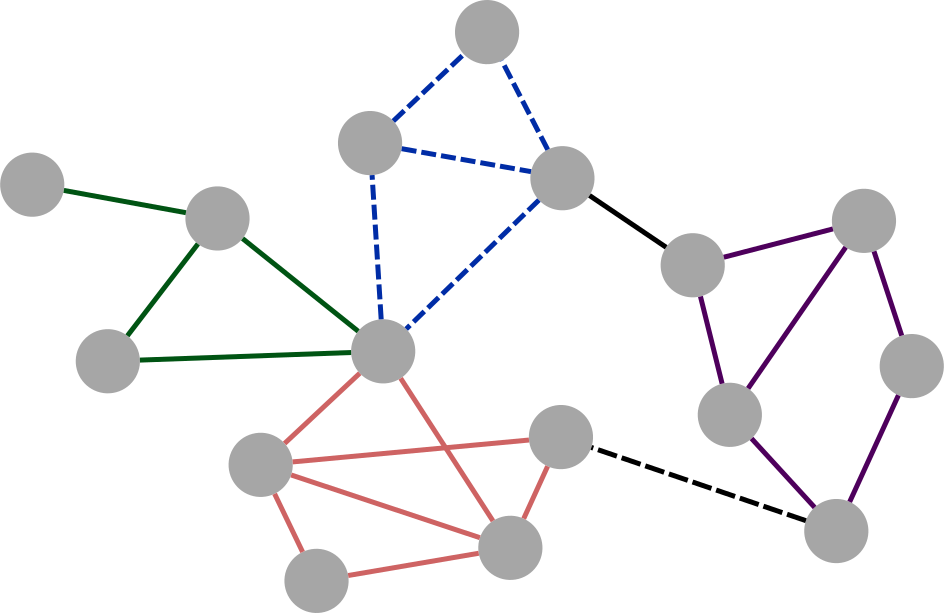
\includegraphics[width=0.5\linewidth]{img/ExpectedNodes/Link_Partition}
\caption{Exemple de de réseau de personne avec une structure communautaire sur les liens qui est représentée par la couleur et le style de chaque lien.}
\label{fig:linkpartition_exemple_expected}
\end{figure}
Afin d'illustrer ce que capture une partition, prenons l'exemple d'un réseau de personnes fictif où le contexte de l'interaction est connue.
Certaines personnes communiquent ensemble car elles sont de la même \textbf{\textcolor{bleu_random}{famille}}, pratiquent le même \textbf{\textcolor{rose_cochon}{sport}}, jouent au \textbf{\textcolor{vert_fonce}{go}} ensemble ou bien encore car elles \textbf{\textcolor{violet_cool}{travaillent}} ensemble.
Nous illustrons cet exemple dans la figure~\ref{fig:linkpartition_exemple_expected} où les interactions sont colorées en fonction de leur contexte.
Il est intéressant de noter que les interactions d'un même type se regroupent ensemble.
Un n\oe ud peut avoir des interactions de plusieurs types, c'est le cas du n\oe ud central qui a des interactions de type \textbf{\textcolor{bleu_random}{famille}}, \textbf{\textcolor{rose_cochon}{sport}} et \textbf{\textcolor{vert_fonce}{go}}.
De même, certaines interactions font le lien entre différent groupes.
C'est le cas du lien pointillé \textbf{noir} qui relie le \textbf{\textcolor{rose_cochon}{sport}} et le \textbf{\textcolor{violet_cool}{travail}} ce qui pourrait se traduire par le financement de l'équipe par l'entreprise.
Ainsi, les partitions de liens peuvent capturer des situations assez variées.

Il est également possible de manipuler des partitions chevauchantes ou couvertures.
Dans ce cas, chaque n\oe ud peut appartenir à plusieurs communautés.
Pour répondre à ce problème de nombreux algorithmes ont été proposés pour la détection et l'évaluation de couvertures de n\oe uds, voir la section~\ref{subsec:cover}.
Les couvertures sont une généralisation des partitions et aucune méthode ne fait encore consensus pour les évaluer car leur structure est complexe, voir la sous-section~\ref{subsec:cover}.
Les partitions de liens, quant à elles, restent des objets plus simples à manipuler.
De plus, elles permettent de mettre en avant une autre structure ayant également du sens.



Il apparait donc les partitions de liens sont des objets à part entières pertinent à étudier.
Pour ce faire, il est nécessaire d'adapter les outils d'analyses pour évaluer directement les partitions de liens.
Nous développons ici une approche similaire à ce qui est fait pour les partitions de n\oe uds et la modularité~\cite{Newman2004}.
Le but est de créer une fonction de qualité permettant d'évaluer une partition de liens d'un graphe.


\section{Travaux existants}
Les notations utilisées sont les suivantes. Soit $G=(V,E)$ un graphe non-orienté avec $V$ l'ensemble des n\oe uds de taille $n$ et $E \subseteq V \times V$ l'ensemble des liens de taille $m$. 
Le degré d'un sommet $u$ de $G$ est noté $d_G(u)$.
Une partition des liens en $k$ groupes est notée $\mathcal{L}=(L_1,L_2,\ldots,L_k)$ avec $L_i \subseteq E \ \forall i$, $L_i\cap L_j=\emptyset \ \forall i\neq j$ et $\bigcup_i L_i=E$.
Pour un groupe de liens $L \in \mathcal{L}$, on pose $V_{in}=\{u \in V, \exists (u,v) \in L\}$ l'ensemble des n\oe uds internes au groupe $L$, $V_{out}=\{u \in V\setminus V_{in}, (u,v) \in E \wedge v \in V_{in} \}$ représente les n\oe uds adjacents au groupe $L$ et enfin $L_{out}=\{(u,v) \in E \setminus L, u \in V_{in} \vee v \in V_{in} \}$ l'ensemble des liens adjacents au groupe $L$ (voir Figure~\ref{fig:example_def_expected}).

\begin{figure}
\centering
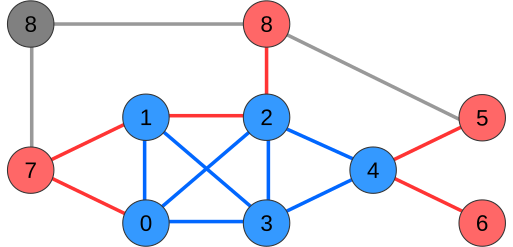
\includegraphics[width=0.4\linewidth]{img/ExpectedNodes/exemple2}
\caption{Exemple d'un groupe de liens $L$ (en \textcolor{semilightblue}{bleu}). Les liens \textcolor{pinkyred}{rouges} sont les liens adjacents $L_{out}$ connectant les n\oe uds internes $V_{in}$ (en \textcolor{semilightblue}{bleu}) aux n\oe uds adjacents $V_{out}$ (en  \textcolor{pinkyred}{rouge}).}
\label{fig:example_def_expected}
\end{figure}

Une approche naïve serait de transformer le graphe initial en un \emph{line-graph}.
Un \emph{line-graph} est un graphe où chaque lien du graphe initial est transformé en un n\oe ud dans le \emph{line-graph}.
Deux n\oe uds du \emph{line-graph} sont reliés si les liens correspondant ont au moins un n\oe ud en commun, voir la figure~\ref{fig:ex_construction_lineG}.
Comme un \emph{line-graph} est un graphe classique, on peut y appliquer toutes les méthodes déjà existantes, \emph{e.g.} les algorithmes de détection de communautés.
Ainsi, une partition des n\oe uds du \emph{line-graph} représente une partition des liens du graphe initiale.
Sur l'exemple~\ref{fig:ex_construction_lineG}, les liens $(1,4)$, $(1,3)$ et $(3, 4)$ du graphe forment un triangle dans le \emph{line-graph} et pourraient être capturés comme étant une communauté.
Ces liens dans le graphe initial forme également un triangle et peuvent être considérés comme une communauté valide.
\begin{figure}
\centering
	\begin{subfigure}{0.25\textwidth}
		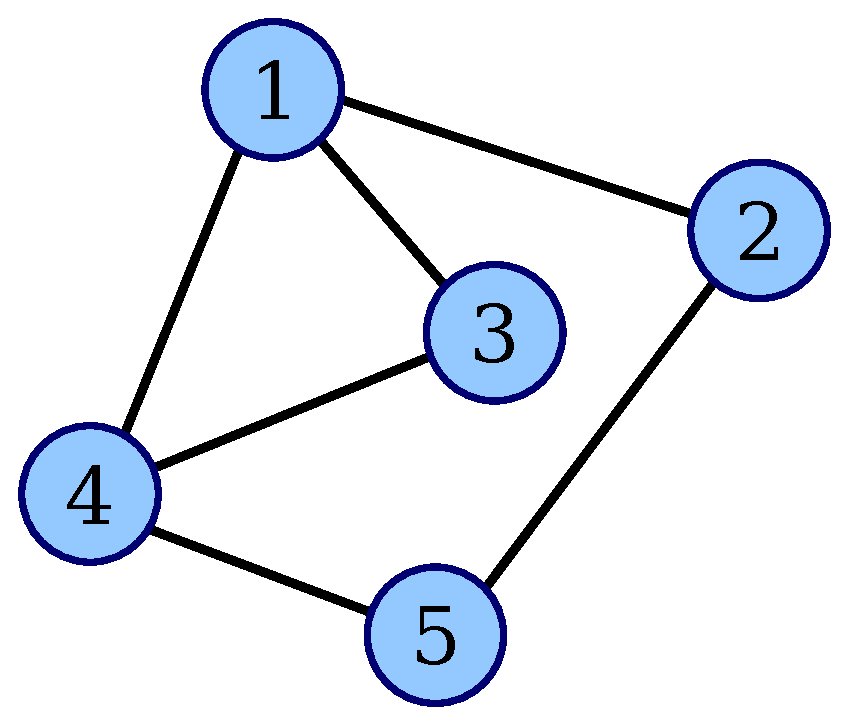
\includegraphics[height=3cm]{img/ExpectedNodes/Line_graph_construction_1.eps}
		\caption{Graphe initial}
	\end{subfigure}\hspace*{0.5cm}
	\begin{subfigure}{0.25\textwidth}
		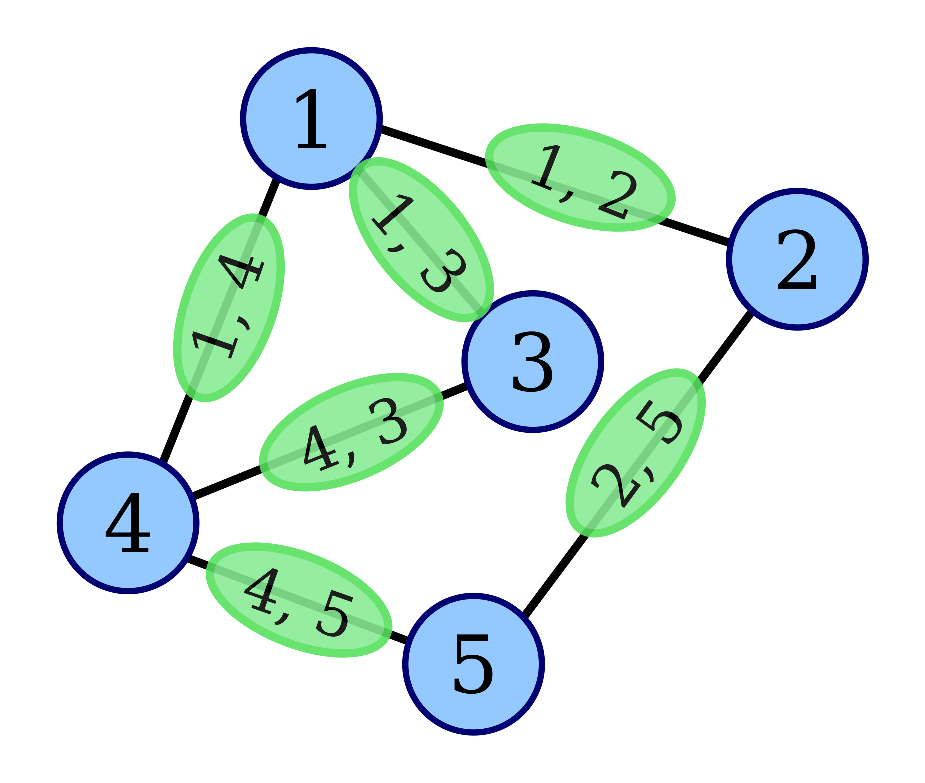
\includegraphics[height=3cm]{img/ExpectedNodes/Line_graph_construction_2.eps}
		\caption{Définition des n\oe uds du \emph{line-graph}}
	\end{subfigure}\hspace*{0.5cm}
	\begin{subfigure}{0.25\textwidth}
		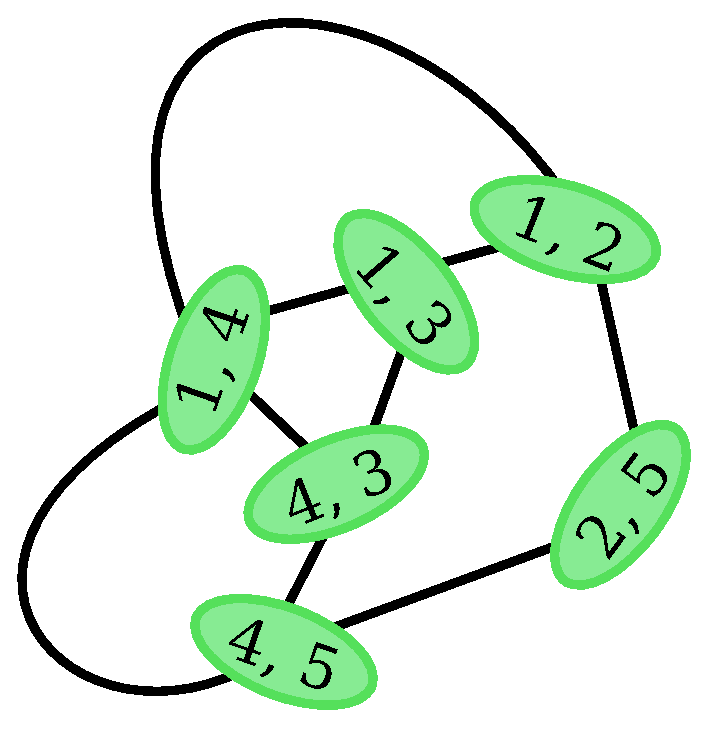
\includegraphics[height=3cm]{img/ExpectedNodes/Line_graph_construction_3.eps}
		\caption{Définition des liens du \emph{line-graph}}
	\end{subfigure}	
	\caption{Exemple de construction du \emph{line-graph}\,\protect\footnotemark.}
	\label{fig:ex_construction_lineG}
\end{figure}
\footnotetext{Image provenant de \url{https://en.wikipedia.org/wiki/Line_graph}.}

Cepdant pour que ce type de méthode fonctionne, il est nécessaire que le \emph{line-graph} résultant puisse être analysé comme un graphe.
En particulier, il est nécessaire que la notion de communauté dans le \emph{line-graph} est un sens dans le graphe initial.
Or, un \emph{line-graph} a une structure très différente du graphe initial.


Prenons pour l'exemple: la clique qui est la meilleur communauté possible et l'étoile qui est une des pires communautés possible.
Le but est d'observer comment ses structures sont transformées dans le \emph{line-graph}.
Ces situations sont représentées dans la figure~\ref{fig:fail_construction_lineG}.
L'étoile dans la figure~\ref{fig:ex_lineG_etoile} est transformée en une clique de 4 n\oe uds.
Une des pires structures communautaires d'un graphe est transformé dans le \emph{line-graph} en la meilleur structure communautaire.
En effet, chaque n\oe uds de degré $k$ du graphe initial donne lieu à une clique de taille $k$ dans le \emph{line-graph}.
Les cliques du \emph{line-graph} ne sont donc pas forcément des communautés dans le graphe.
Dans le cas de la clique $4$ dans la figure~\ref{fig:ex_lineG_clique}, on remarque que le \emph{line-graph} est composé de $6$ n\oe uds et de uniquement $12$ liens.
Plus généralement une clique de taille $n$ dans le graphe initial donne lieu dans le \emph{line-graph} à $\dfrac{n(n-1)}{2}$ n\oe uds et $(n-1)n$ liens.
Ainsi, plus la clique est grande dans le graphe, moins la structure résultante dans le \emph{line-graph} est dense.
Les cliques du graphe sont donc moins denses que ses étoiles, lorsqu'on les observe dans le \emph{line-graph}.

Il n'est donc pas innocent d'utiliser le \emph{line-graph} pour trouver des communautés de liens.
Il est nécessaire d'adapter les outils à ce type de graphe.
\begin{figure}
\centering
	\hfill
	\begin{subfigure}{0.4\textwidth}
		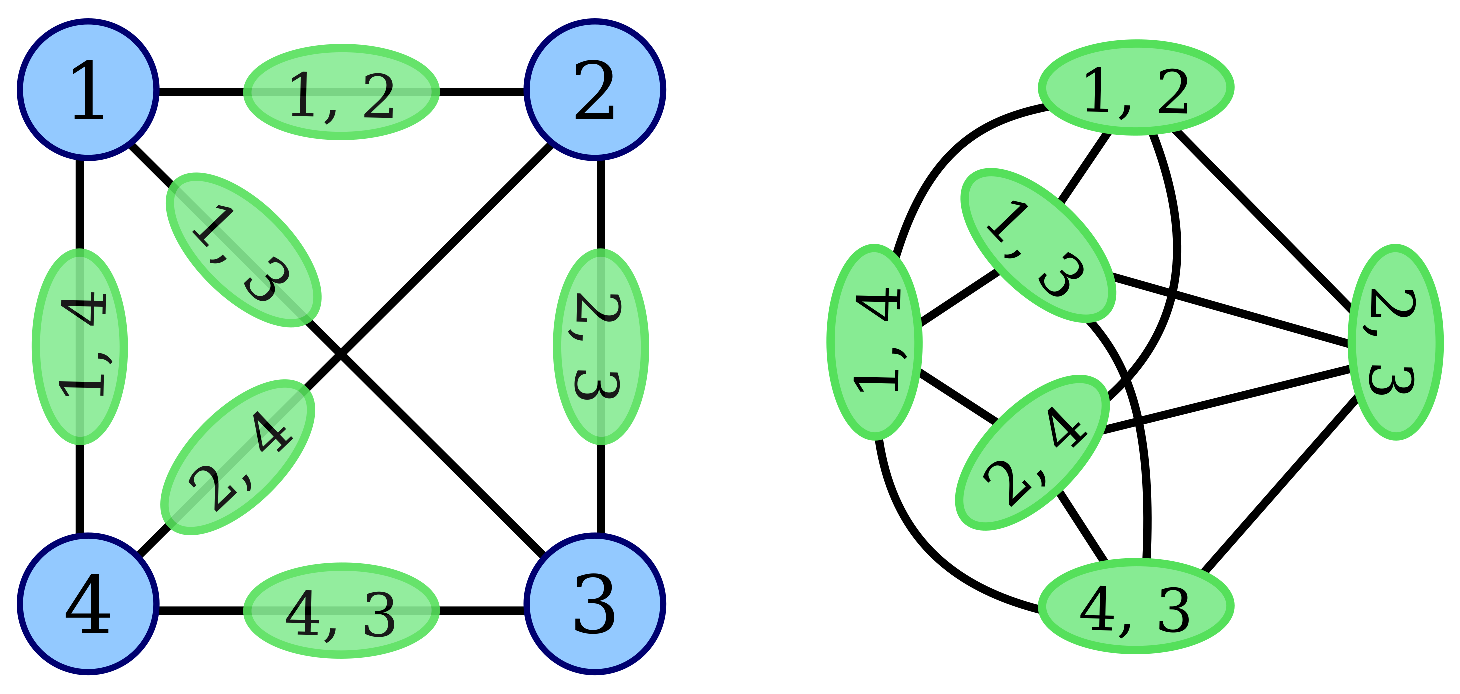
\includegraphics[height=3cm]{img/ExpectedNodes/Example/transfo_clique}
		\caption{}
		\label{fig:ex_lineG_clique}	
	\end{subfigure}\hfill
	\begin{subfigure}{0.4\textwidth}
		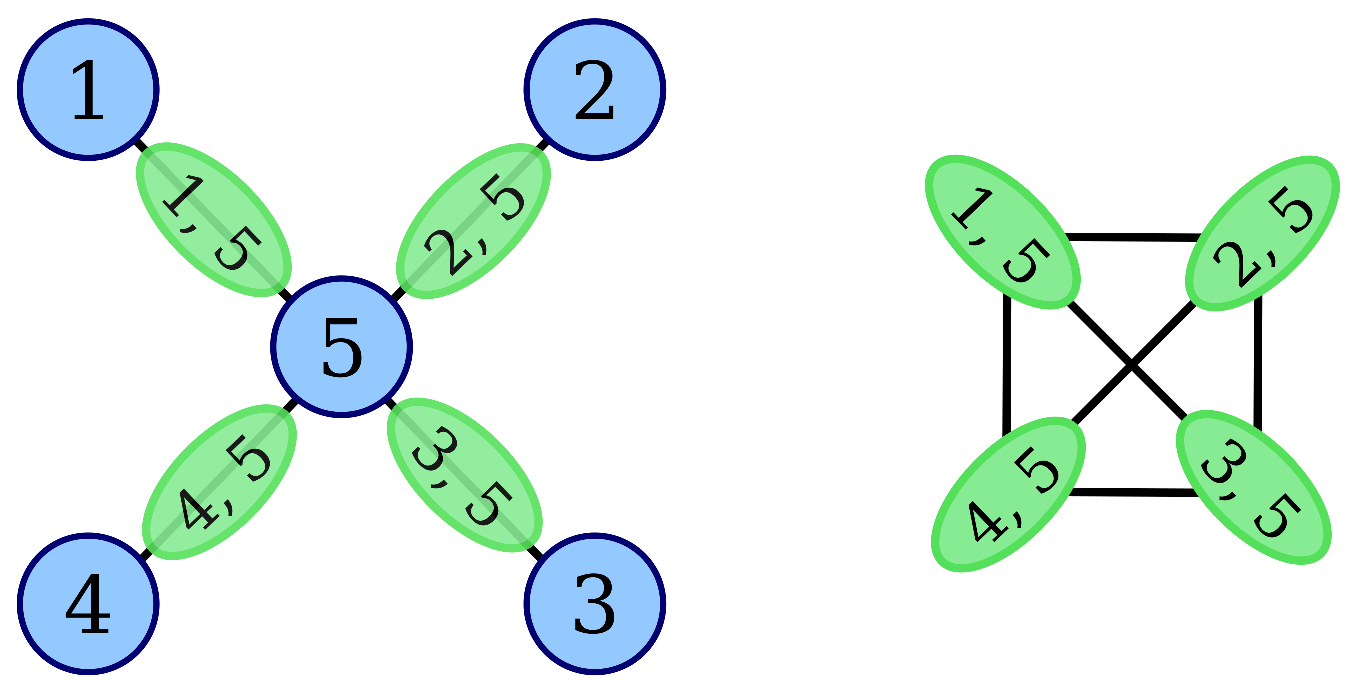
\includegraphics[height=3cm]{img/ExpectedNodes/Example/transfo_etoile}
		\caption{}
		\label{fig:ex_lineG_etoile}	
	\end{subfigure}
	\hfill		

	\caption{Exemple de construction du \emph{line-graph} d'une clique en (A) et d'une étoile en (B).}
	\label{fig:fail_construction_lineG}
\end{figure}



Il existe différent types de méthode pour la détection et l'évaluation de partitions de liens.
Il y les méthodes évaluant une partition de liens via la transformation de la partition en une couverture de n\oe uds~\cite{Huang2013,Lim2014,Wu2010a}.
Un transformation classiquement utilisée est qu'un n\oe ud dans la couverture prend comme communautés l'ensemble des communautés de ses liens, voir la figure~\ref{fig:Partition_Couverture}.
Il serait tentant de considérer que les partitions de liens et les couvertures de n\oe uds sont équivalentes.
Ainsi pour évaluer une partition de liens, il suffirait de transformer la partition en couverture.
Or, ce changement n'est pas anodin.
D'une part, les couvertures de n\oe uds permettent de modéliser beaucoup plus de situations car il n'y a aucune contrainte sur les couvertures.
D'autre part, il n'est pas trivial de transformer une partition de liens en couverture de n\oe uds, et \emph{vice versa}.

\begin{figure}
\centering
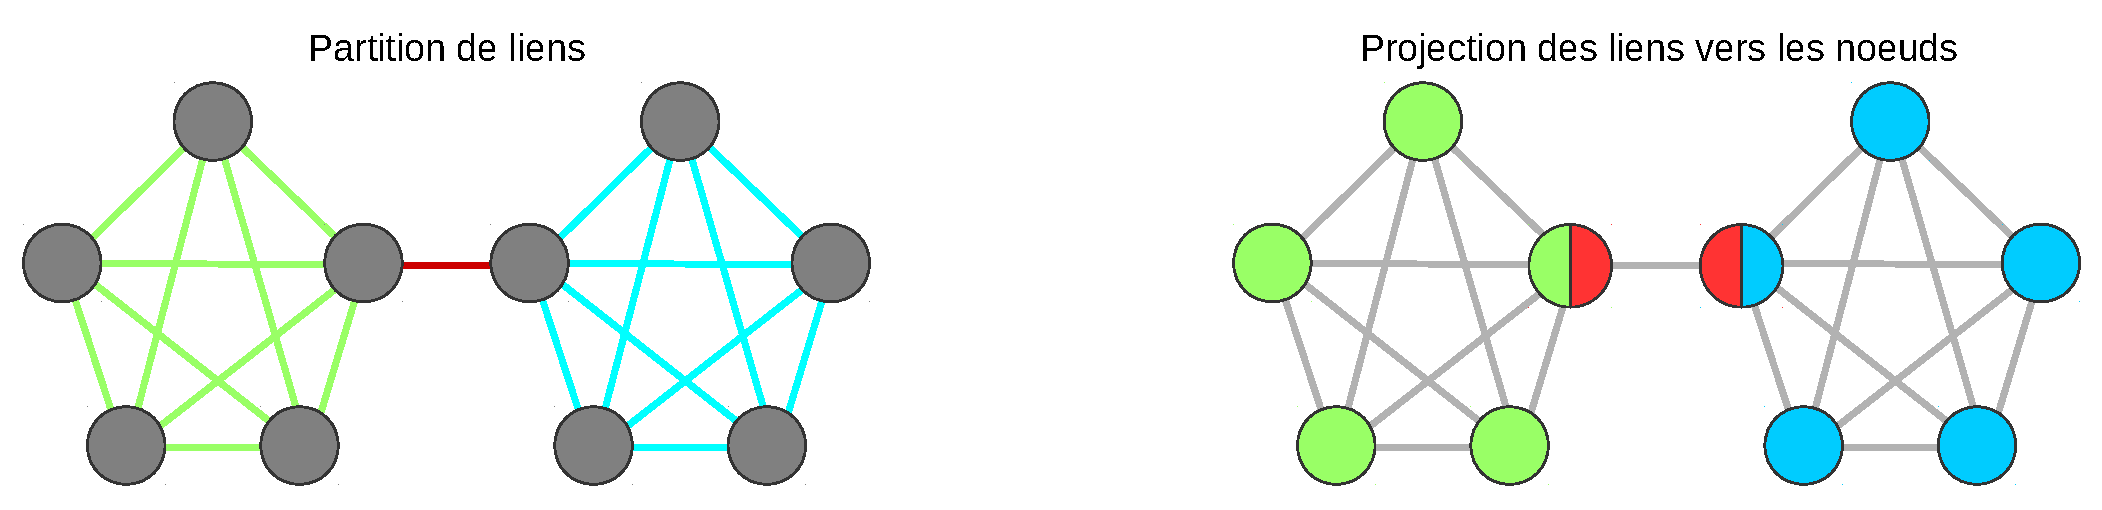
\includegraphics[width=0.9\linewidth]{img/ExpectedNodes/Partition_Couverture}
\caption{Transformation d'une partition de liens à gauche en couverture de n\oe uds à droite. La couleur représente un groupe.}
\label{fig:Partition_Couverture}
\end{figure}


Dans l'exemple de la figure~\ref{fig:Partition_Couverture}, il n'est évident pas que la communauté \textcolor{briquered}{\textbf{rouge}} constituée des deux n\oe uds centraux soit une communauté légitime.
Selon le contexte, elle peut être considérée comme un artefact de la transformation.
La transformation d'une partition n'est donc pas un acte neutre.
Cet aspect a d'ailleurs été mis en avant par Esquivel~\emph{et al}~\cite{Esquivel2011}.
Face à ce problème, nos travaux ainsi que quelques méthodes existantes proposent des méthodes évaluant directement les partitions de liens.

Ahn~\emph{et al.}~\cite{Ahn2010a} sont parmi les premiers à avoir proposé une méthode détectant les communautés de liens.
Leur méthode \emph{link clustering} est une méthode hiérarchique d'agglomération.
Elle construit un dendrogramme en agglomérant de manière itérative les groupes de liens en fonction de leur similarité calculée par l'indice de Jaccard.
Afin de décider de la coupe du dendrogramme et de la partition résultante, la fonction \emph{Partition Density} est utilisée.
Pour une partition de liens donnée $\mathcal{L}$, la \emph{Partition Density} est définie de la manière suivante:
\begin{equation}
D(\mathcal{L}) = \dfrac{\sum_{L \in \mathcal{L}} |L|D(L)}{m} \quad D(L) = \dfrac{|L|- min_D(|V_{in}|) }{max_D(|V_{in}|) - min_D(|V_{in}|)},
\end{equation}

où $min_D(N) = N - 1$ est le nombre minimum de liens pour relier $N$ n\oe uds et $max_D(N) = \dfrac{N(N - 1)}{2}$ est le nombre maximum de liens qu'il puisse exister entre $N$ n\oe uds.
Malgré son nom la \emph{Partition Density} n'est pas une densité mais le nombre de liens du groupe normalisé par le nombre de liens minimum et maximum pour un groupe de $|V_{in}|$ n\oe uds.
\\
Après simplification, on obtient la formule suivante:

\begin{equation}
 D(L) = 2 \dfrac{|L| - (|V_{in}|-1) }{(|V_{in}|-1) (|V_{in}|-2)}.
\end{equation}

Par convention, un groupe constitué d'un unique lien, et qui n'a donc que deux n\oe uds internes, a une qualité nulle.

D'autres chercheurs~\cite{Li2013,Shi2013} ont par la suite utilisé la \emph{Partition Density} comme fonction à optimiser dans des algorithmes génétique.
Leurs solutions semblent pour l'instant difficilement utilisable car leurs algorithmes reposent sur de nombreux critères et sont limités à de petit graphes.

Par ailleurs, la \emph{Partition Density} ne peut pas être directement appliquée aux graphes pondérés.
Une première proposition de Kim~\cite{Kim2014} a été faite dans ce sens.


Evans~\emph{et al.}~\cite{Evans2009} proposent trois fonctions de qualité pour évaluer les partitions de liens.
Leurs fonctions de qualité sont basées sur trois marches aléatoires qui se déroulent sur les liens du graphe.
L'approche est similaire à la modularité car la modularité peut également être définie à l'aide de marche aléatoire sur les n\oe uds du graphe~\cite{Delvenne2010}.
Leurs trois fonctions de qualité peuvent être calculées et optimisées sur le graphe mais les auteurs ont montré que l'on pouvait, de manière complètement équivalente, utiliser la modularité sur des \emph{line-graph} pondérés ($LG_1$, $LG_2$, $LG_3$).
Ainsi, il suffit de construire le \emph{line-graph} approprié puis d'utiliser un algorithme existant d'optimisation de la modularité tel que l'algorithme de \emph{Louvain}~\cite{Blondel2008a}.


Pour construire les \emph{line-graphs}  $LG_1$, $LG_2$ et $LG_3$, nous définissons $B\in \mathcal{M}_{n,m}$ la matrice d'incidence du graphe $G$: un élément $B_{i\alpha}$ de cette matrice $|V| \times |E|$ est égale à $1$ si le lien $\alpha$ est relié au n\oe ud $i$ et 0 sinon.
Les matrices $LG_1$, $LG_2$ et $LG_3$ sont alors définies de la manières suivante:
\begin{center}
	\begin{tabular}{|c|c|c|c|}
		\hline  & $x=1$ & $x=2$ &  $x=3$\\ 
		\hline \rule{0pt}{1.7em} $LG_x(\alpha,\beta)$ & $B_{i\alpha}B_{i\beta} (1-\delta_{\alpha \beta})$ & $\sum_{i \in V, d_G(i)>1}\dfrac{B_{i\alpha}B_{i\beta}}{d(i)-1}$ & $\sum_{i,j \in V, d(i)d_G(j)>0}\dfrac{B_{i\alpha}A_{ij}B_{j\beta}}{d(i)d(j)}$ \\
		\hline 
	\end{tabular} 
\end{center}
Soit $k_x(\alpha)= \sum_{\beta}LG_x(\alpha,\beta)$ le degré pondéré dans le line graphe $LG_x$ du n\oe ud représentant le lien $\alpha$ et $W_x = \sum_{\alpha,\beta \in |E|}LG_x(\alpha,\beta)$ la somme des poids des liens. Pour $x \in \{1,2,3\}$, la fonction de qualité $Evans_x$ est définie de la manière suivante:
\begin{eqnarray}
Evans_x(\mathcal{L}) = \dfrac{1}{W_x} \sum_{L_i \in \mathcal{L}} \sum_{e_1,e_2 \in L_i^2} LG_x    (e_1,e_2) -  \dfrac{k_x(e_1) k_x(e_2)}{W}.
\end{eqnarray}

Kim \emph{et al.}~\cite{Kim2011} ont exploré une extension du concept de \emph{Minimum Length Description} (MDL) introduit par Rosvall~\emph{et al.}~\cite{Rosvall2008} qui est une méthode provenant de la théorie de l'information.
Cette extension de la \emph{MDL} évalue directement une partition de liens, contrairement à l'extension proposée par Esquivel~\emph{et al.}~\cite{Esquivel2011}.
Un avantage de leur méthode est de pouvoir comparer la qualité d'une partition de liens et d'une partition de n\oe uds avec leur \emph{MDL} respective.
Cependant, leur méthode ne semble favoriser les communautés de liens que dans des cas très limités.

Pour résumer, il existe des méthodes pour capturer et évaluer des partitions de liens dans un graphe.
Deux d'entre elles semblent faire consensus pour l'instant.
D'une part, la \emph{Partition density} est une fonction de qualité comparant le nombre de liens observé avec les nombres minium et maximum de liens possibles entre les même n\oe uds induits.
D'autre part, les fonctions de qualité \emph{$Evans_x$} se basent quand à elles sur des marches aléatoires sur les liens et d'une certaine manière sur un processus similaire à la modularité.
Il n'existe cependant aucune méthode utilisant une comparaison d'une métrique à ce qui est attendu dans un modèle nul.
Or, ce processus a été à l'origine de la modularité.

\section{Définition d'Expected Nodes}

Une idée souvent utilisée lors de la détection de communautés de n\oe uds est qu'une communauté devrait avoir beaucoup de connexion en interne.
Pour évaluer ce genre de définition intuitive, il est nécessaire de définir à quoi comparer le nombre de connexions interne.
Le choix qui est fait avec la modularité et d'autres méthodes est de définir un modèle nul aléatoire où il n'existe pas de structure communautaire.
Le but est de construire un graphe aléatoire qui partage un certain nombre de caractéristiques avec le graphe initial mais dont la structure communautaire a été détruite lors du mélange.

Il existe de nombreux modèles et celui utilisé dans la modularité est le modèle de configuration~\cite{Bender1978a}.
Dans ce modèle, le nombre de n\oe uds et leurs degrés sont fixes mais la répartition des liens est aléatoire.
Ainsi pour chaque n\oe ud, ses voisins sont tirés de manière aléatoire avec une probabilité proportionnelle à leur degré.
Comme les liens sont mélangés dans ce modèle, on suppose qu'il n'existe plus de structure communautaire dans le graphe.

Pour notre fonction de qualité \emph{Expected Nodes}, nous utilisons également le modèle de configuration.
Avant d'aller plus loin et de définir formellement \emph{Expected Nodes}, il est utile d'avoir une définition informelle de la fonction de qualité.

Le but est d'évaluer un groupe de liens.
Afin qu'un groupe de liens soit évalué comme une bonne communauté, les liens devraient induire un nombre relativement faible de n\oe uds internes.
En effet, plus le nombre de n\oe uds internes est faible, plus le groupe de liens ressemble à une clique.
De manière similaire à la modularité, nous utilisons le configuration modèle pour calculer le nombre de n\oe uds interne espéré dans le modèle de configuration.
Si le groupe de liens a moins de n\oe uds internes qu'espéré alors ça indique que le groupe de liens est plus dense et qu'il devrait donc avoir une évaluation élevée.

Il est donc nécessaire de calculer l'espérance du nombre de n\oe uds interne, $\mu_{G}$, d'un groupe de liens, $L$, dans le modèle nul.
Un n\oe ud de $G$ est interne si au moins un de ses liens appartient à $L$.
Ainsi pour calculer $\mu_{G}$, il faut tirer aléatoirement et sans remise $2|L|$ demi-liens parmi les $2|E|$ demi-liens du  graphe aléatoire avec la même distribution de degrés.
Soit $B_u$ la variable aléatoire correspondant au nombre de fois où le n\oe ud $u$ est tiré.
Cette variable suit une loi  hypergéométrique $B_u \sim \mathcal{G}\left(2|E|,d_G(u),2m\right)$.
Avec cette notation, on définie $\mu_G$ de la manière suivante:

\begin{equation}
\label{eq:nbsommet_esp} \mu_{G}(|L|) = \sum_{u\in V} \mathbb{P}( B_u \geq 1 )
=  \sum_{u \in V} 1 - \dfrac{ \binom{2|E|-d(u)}{2|L|} }{ \binom{2|E|}{2|L|} }. 
\end{equation}

Voici quelques propriétés de la fonction $\mu_{G}(|L|)$ :
\begin{itemize}
\item La fonction $\mu_{G}$ dépend uniquement de la séquence de degrés $\{d_G(v)\}_{v \in V}$ et du nombre de liens.
%On peut montrer que cette fonction est Schur-concave, ainsi plus les degrés sont uniformément répartis plus il sera surprenant d'observer un groupe de liens correspondant à peu de n\oe uds.
\item Pour une distribution de degrés donnée, la fonction   $\mu_{G}(|L|)$ est une fonction croissante de $|E|$.
\item Si $L=E$, alors le nombre de n\oe uds attendus est bien égal à $|V|$.
\item On a $\mu_{G}(1)\leq 2$, en effet le modèle nul n'interdit pas la présence de boucle.
\end{itemize}

Avec $\mu_G$, nous pouvons définir la qualité \emph{interne}, $Q_{in}$ d'un groupe de liens $L$:
  
\begin{equation}
\label{eq:qin} Q_{in}(L) = \dfrac{\mu_{G}(|L|) - |V_{in}(L)|}{\mu_{G}(|L|)}.
\end{equation}

Avec cette formulation, pour un groupe de taille $|L|$, plus le nombre de n\oe uds internes est faible, plus $Q_{in}$ sera élevée.

$Q_{in}$ permet d'évaluer la qualité interne d'un groupe mais il faut aussi tenir compte du voisinage.
En effet, observer une clique a l'intérieur d'une autre clique n'est absolument pas surprenant.
C'est pourquoi, nous définissons également une qualité externe.
Le but est d'évaluer comment sont répartis les liens et n\oe uds adjacents.
Pour ce faire, nous allons également comparer le nombre de n\oe uds adjacents observé au nombre espéré dans le modèle de configuration.
Cependant à l'inverse de la qualité interne, la qualité externe est \textbf{mauvaise} si jamais le nombre de n\oe uds adjacent est plus faible qu'espéré.
En effet, si il y a beaucoup de liens adjacents pour peu de n\oe uds, alors cela indique que le voisinage du groupe est dense et devrait être inclus dans le groupe.
Le cas idéal est que chaque lien adjacent soit relié à un n\oe ud différent.

Soit $\bar{d}(L,u) = \sum_{v \in V} \mathbf{1}_{(u,v) \in E \setminus L}$ le degré de $u$ limité aux liens adjacents et $\bar{d}(L)=\sum_{u \in V_{in}(L)} \bar{d}(L,u)$.
L'espérance du nombre de n\oe uds adjacents est calculé comme le nombre de n\oe uds tirés lorsque $\bar{d}(L)$ demi-liens sont choisis aléatoirement et sans remise dans le modèle de configuration où les liens de $L$ ont été préalablement retirés.
Ce graphe aléatoire a la distribution de degrés suivante: $\{d_{G \setminus L }(u)\}_{u \in V}$ où $G \setminus L = (V,E\setminus L)$.
Dans ce cas, on ne tire pas aléatoirement un lien mais uniquement un demi-lien car l'autre demi-lien est un des demi-liens reliés aux n\oe uds internes.
L'espérance du nombre de n\oe uds adjacents se définit de la manière suivante:

\begin{equation}
	\mathbb{E}[\bar{d}(L)] = \mu_{G\setminus L}(\bar{d(L)}/2).
\end{equation}

Une illustration de ce processus est présentée dans la figure~\ref{fig:retourt_ext}.
Sur cette illustration, le groupe $L$ a un très mauvais voisinage et cela se reflète par un nombre de n\oe uds adjacents observés plus faible qu'espéré.

\begin{figure}
\centering
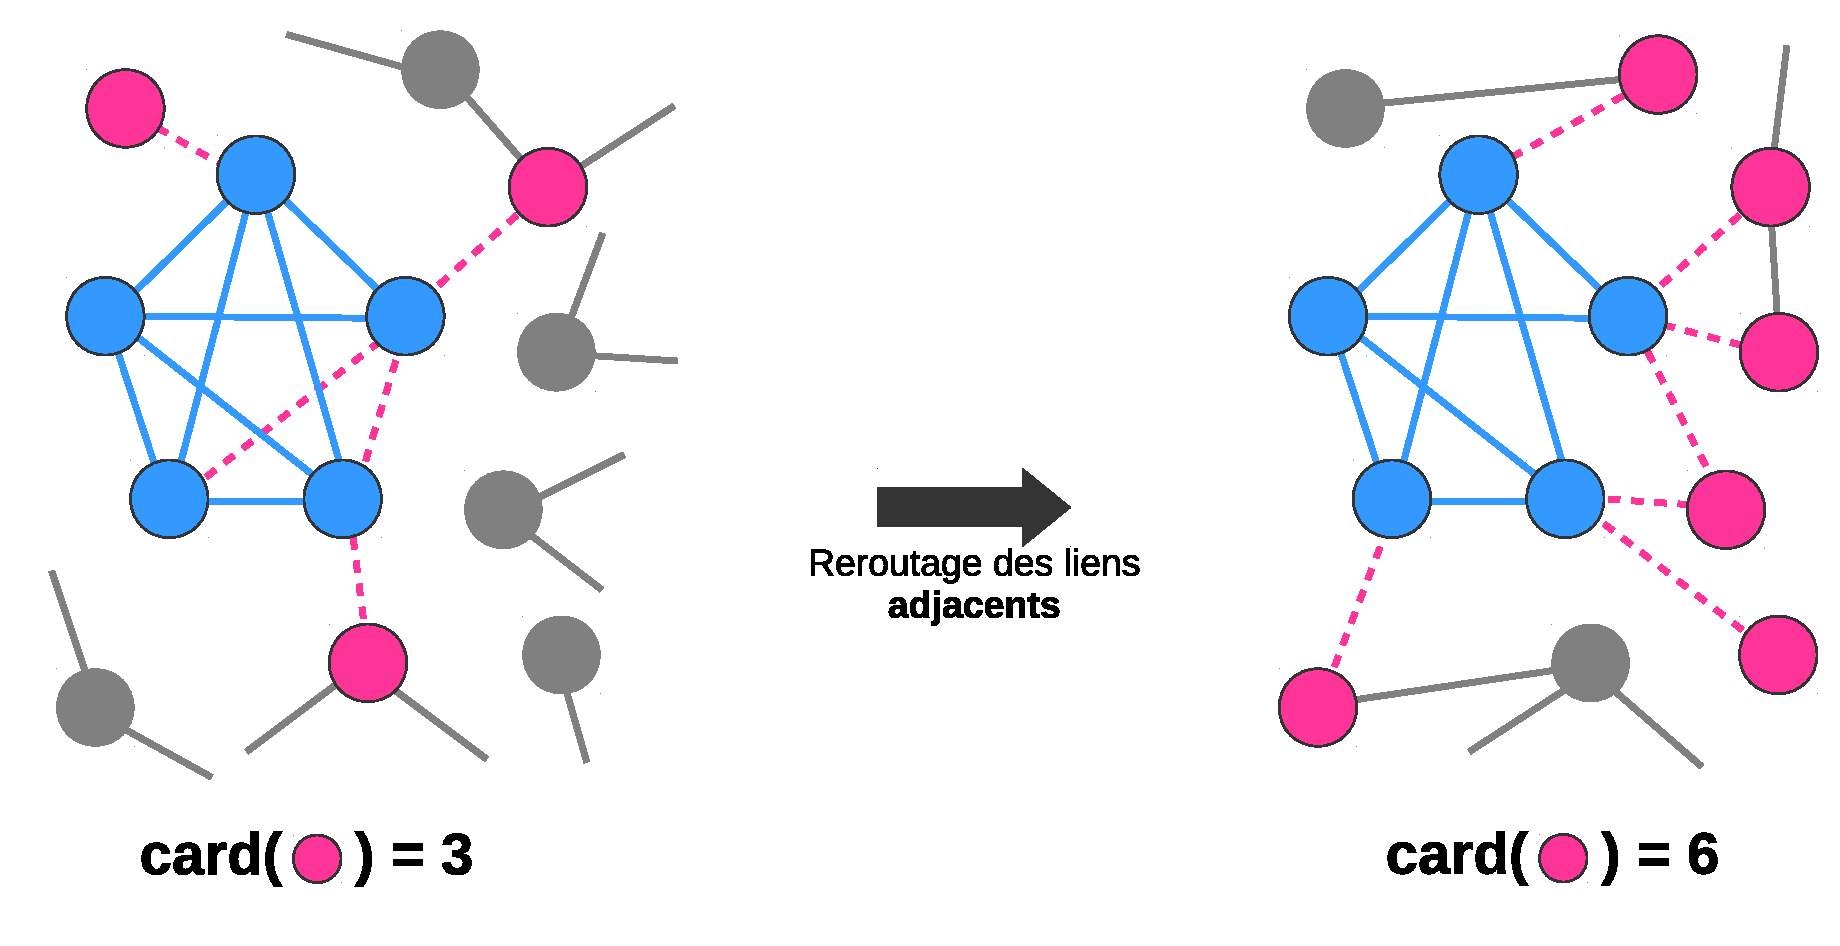
\includegraphics[width=0.7\linewidth]{img/ExpectedNodes/reroutageExt3}
\caption{Groupe de liens $L$ en \textcolor{semilightblue}{\textbf{bleu}} et ces liens adjacents en \textcolor{pinkyred}{\textbf{rose}} pointillés dans le graphe initial à gauche.
\`A droite, une réalisation du modèle de configuration où $L$ a été figé.}
\label{fig:retourt_ext}
\end{figure}

Comme il est intéressant de pénaliser les groupes ayant de mauvais voisinage mais qu'un bon voisinage n'est pas suffisant pour définir une bonne communauté, nous bornons à $0$ la qualité externe:

\begin{equation}
\label{eq:qext} Q_{ext}(L) = min \left(0, \dfrac{|V_{out}(L)| - \mu_{G\setminus L}(\bar{d}(L)/2)}{\mu_{G\setminus L}(\bar{d}(L)/2)} \right).
\end{equation}


Enfin, nous définissons \emph{Expected Nodes} pour un groupe $L$:
\begin{equation}
	\label{eq:qAlg}
	Q(L)  =  2\dfrac{ |L|Q_{in}(L) + |L_{out}|Q_{ext}(L)}{|L|+|L_{out}|}.
\end{equation}

La qualité interne est due aux liens de $L$ et la qualité externe aux liens adjacents.
C'est pourquoi nous pondérons $Q_{in}$ par $|L|$ et $Q_{ext}$ par $|L_{out}|$.



Nous détaillons maintenant certaines propriétés des formules \ref{eq:qext} et \ref{eq:qAlg} découlant des propriétés de $\mu_{G}$ en nous appuyant sur des exemples.
En s'intéressant aux n\oe uds adjacents $V_{out}$, on pénalise la présence de n\oe uds adjacents fortement connectés avec les n\oe uds incidents à $L$.
Prenons le cas extrême où $L$ est une clique qui est incluse dans une plus grande clique alors que le reste du graphe est quelconque.
Dans cette situation, $Q_{in}(L)$ est maximum car le groupe est une clique.
En revanche, $Q_{ext}(L)$ va fortement pénaliser la qualité du groupe car il y a dans ce cas beaucoup de liens adjacents pour très peu de n\oe uds adjacents.
Ainsi, la $Q_{ext}$ permet de pénaliser les n\oe uds adjacents ayant beaucoup de liens avec $L$.
L'idée est que ces liens adjacents devraient être intégrés à $L$.

Bien évidement, la solution n'est pas de systématiquement d'intégrer les liens adjacents car intégré un lien adjacent peut également faire baisser $Q_{in}$.
Par exemple, un lien reliant deux groupes denses disjoints peut avoir une qualité positive.
Cette situation est visible dans la figure~\ref{fig:Partition_Couverture} partie gauche.
Ce lien tout seul a d'une part une qualité interne positive car $\mu_G(1) \leq 2$ et d'autre part il a une qualité externe nulle car chaque n\oe ud adjacent n'est relié qu'à un seul lien adjacent ce qui est le cas idéale.
Dans une situation plus générale, la qualité d'un lien isolé dépend du nombre de triangles dans lequel il se trouve.
Moins le nombre de triangle est élevé, meilleure sera la qualité externe.

Enfin il est intéressant de noter que la qualité du groupe contenant tout les liens est nulle.
En effet comme dit précédemment, $Q_{in}(E)$ égal à zéro, voir l'équation \ref{eq:nbsommet_esp}.
De plus, si le groupe contient tout les liens alors il n'y a plus de liens adjacents et donc seule  $Q_{in}(E)$ influe sur $Q(E)$.



Nous définissons \emph{Expected Nodes} pour une partition de liens $\mathcal{L}$ comme la moyenne pondérée de la qualité de chaque groupe:
\begin{equation}
\label{eq:qualite_globale} Q_G(\mathcal{L}) = \dfrac{\sum_{L\in \mathcal{L}} |L|Q(L)}{|E|}.
\end{equation}

D'autres choix de pondération pour $Q_{in}$, $Q_{ext}$ et $Q_G$ ont été testés en utilisant le nombre de n\oe uds au lieu du nombre de liens mais elles ont été abandonnées lors des tests qui sont présentés dans la section~\ref{sec:expected_comp}.

\section{Comparaison}
\label{sec:expected_comp}
Nous évaluons maintenant \emph{Expected Nodes} en utilisant deux jeux de test.
Sur ces jeux de tests, nous appliquons également des fonctions de qualités reconnues:
\emph{Partition Density}~\cite{Ahn2010a} et les fonctions de qualité proposées par Evans \emph{et al.}~\cite{Evans2009} que nous nommons $Evans1$, $Evans2$ et $Evans3$.
Pour chaque graphe de test, nous créons empiriquement plusieurs partitions de liens et nous évaluons chaque partition avec toutes les fonctions de qualité.

\subsection{Cas du graphe complet}
\label{Completegraph}
Le premier jeu de test est assez simple puisqu'il s'agit d'un graphe complet.
Le but est de vérifier que \emph{Expected Nodes} n'a pas un comportement dégénéré.
Nous étudions un graphe complet de $100$ n\oe uds\,\footnote{Nous avons obtenus des résultats similaires pour un graphe de $500$ n\oe uds.}.
Sur ce graphe, nous définissons plusieurs partitions.
La première est la partition triviale où tout les liens sont dans un unique groupe.
Nous définissons également deux familles de partitions: une séparant les liens en deux groupes et une séparant les liens en 3 groupes.
Soit $V'$ un ensemble de $p$ n\oe uds où $p$ est un paramètre $p<|V|$.
Les deux familles de partitions placent les liens de $V' \times V'$ dans un groupe.
Pour la partition en 2 groupes, tout les autres liens sont mis dans un second groupe.
Pour la partition en 3 groupes, les liens de $V \times V\setminus V'$ sont dans un second groupe et le reste dans un troisième.
Ces répartitions sont illustrées dans la figure~\ref{fig:1C}.

\begin{figure}
\centering
	\begin{subfigure}{0.2\linewidth}
		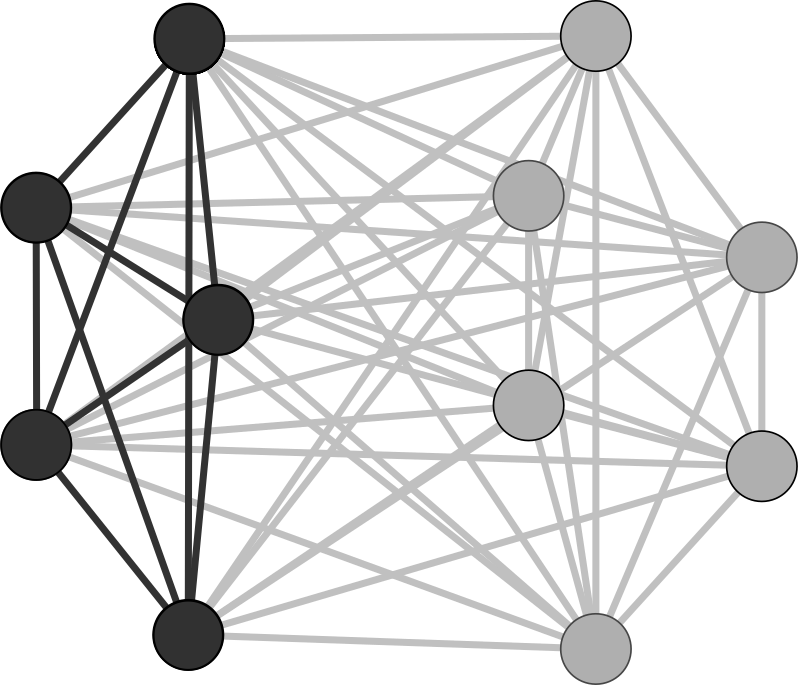
\includegraphics[width=\linewidth]{img/ExpectedNodes/1Clique/Clique2}
		\caption{\label{fig:1C2}}	
	\end{subfigure}	\hspace{2cm}
	\begin{subfigure}{0.2\linewidth}
			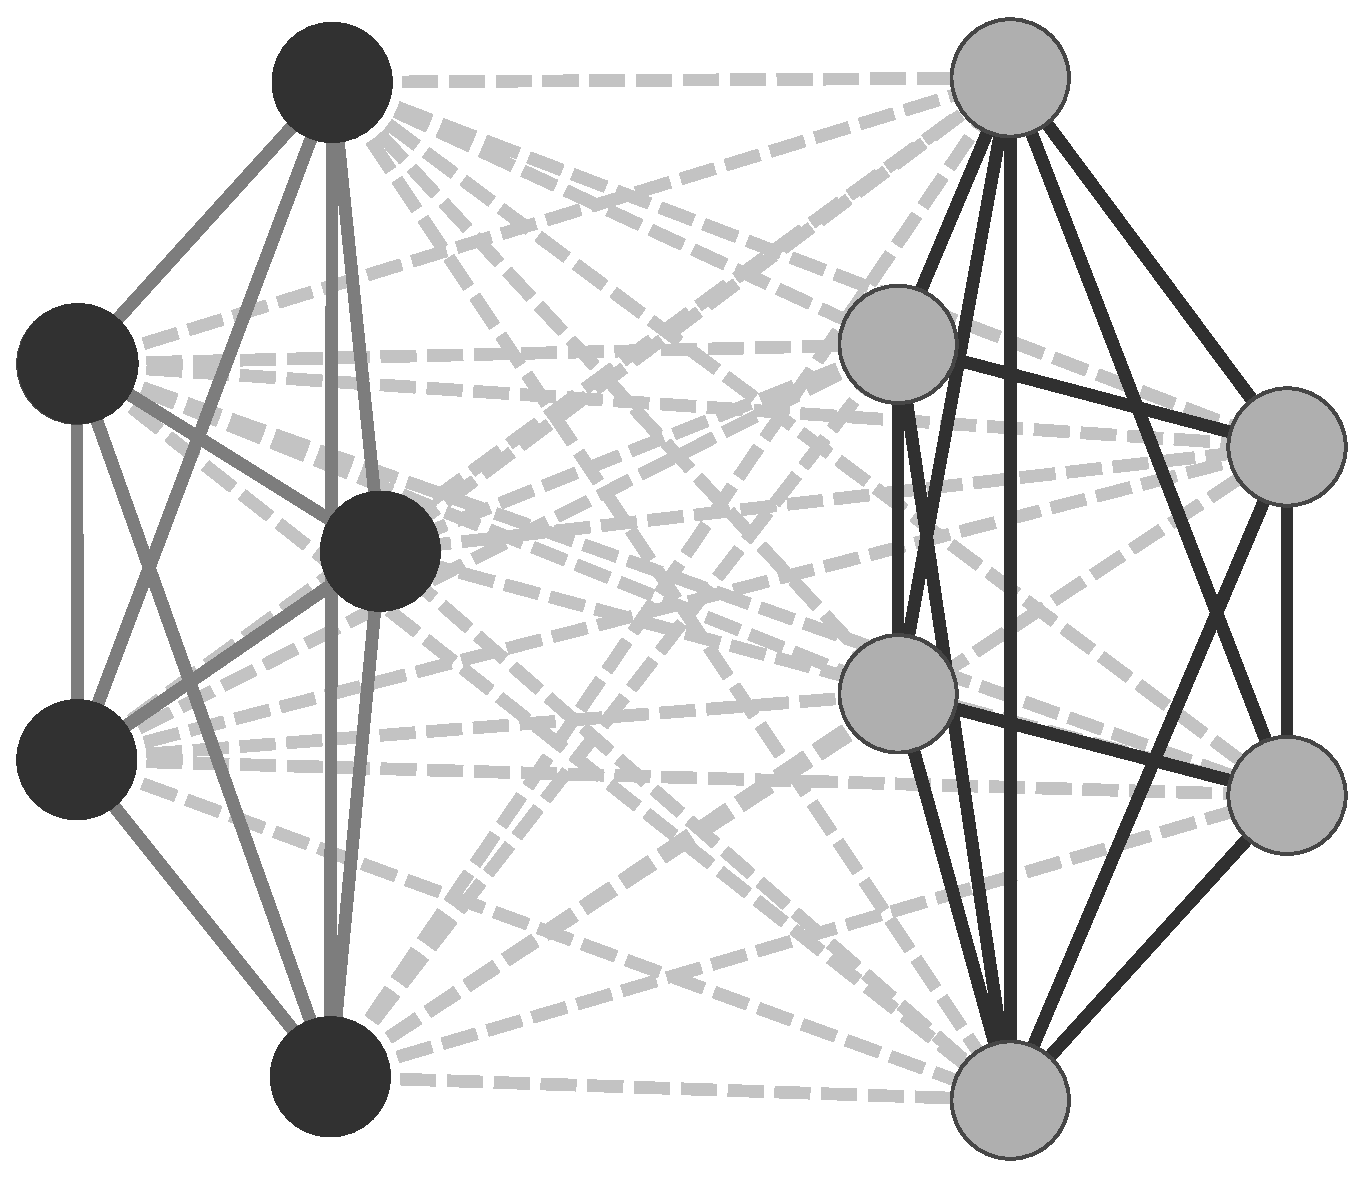
\includegraphics[width=\linewidth]{img/ExpectedNodes/1Clique/Clique3}
			\caption{\label{fig:1C3}}		
	\end{subfigure}
	\caption{Deux partitions de liens pour un graphe complet à $10$ n\oe uds avec $p=5$: (a) partition en deux groupes et (b) partition en trois groupes.
	Les n\oe uds noirs sont les n\oe uds appartenant à $V'$ et la couleur d'un lien correspond à son groupe.}
	\label{fig:1C}
\end{figure}


Comme le graphe est un graphe complet, la meilleur solution est d'avoir un seul groupe contenant l'ensemble des liens, \textit{i.e.} la partition triviale devrait avoir une meilleur évaluation que les autres partitions.
La figure~\ref{fig:1Cres} présente les résultats.
Pour chaque valeur de $p$ et chaque fonction de qualité, nous calculons les évaluations des partitions en deux et en trois groupes ainsi que l'évaluation de la partition triviale.
L'évaluation de la partition triviale n'est pas dépendante de $p$ et n'est calculée qu'une seule fois.
Tout d'abord, la construction de cet exemple est symétrique pour la partition en deux groupes.
En effet, la partition en eux groupes lorsque $p$ égal $24$ est complètement équivalente à la partition en deux groupes lorsque $p$ égal $76$.
Par ailleurs, il est possible de définir formellement la qualité de  chacune de ses partitions selon toutes les fonctions de qualité.
Cependant, la complexité des équations, surtout pour \emph{Expected Nodes} et $Evans_x$, rend le résultat difficilement interprétable.


De manière assez surprenante, les fonctions $Evans1$ et $Evans2$ ne passent pas ce test car elles évaluent la partition en deux ou trois groupes comme meilleure que la partition triviale.
Selon la \emph{Partition Density}, \emph{Expected Nodes} et $Evans3$, la partition triviale est la meilleur des partitions.
La fonction $Evans3$ diffère légèrement des deux autres car elle a une amplitude plus faible ($\approx 10^{-3}$).

%\begin{equation}
%Expected\_nodes(p) = \dfrac{1}{C(100)}(C(p) Q(L_{gauche}) + C(100-p) Q(L_{droite}))
%\end{equation}
%\begin{equation}
%Q(L_{gauche})= 2\dfrac{C(p) 100 (1 - \dfrac{ \binom{2C(100) - 99}{2C(p)} }{ \binom{2C(100)}{2C(p)} }) - (100-p)p }{C(p)+ (100-p)p}
%\end{equation}
%$C(p)= \dfrac{p(p-1)}{2}$

\begin{figure}
\centering
	\begin{subfigure}{0.4\linewidth}
		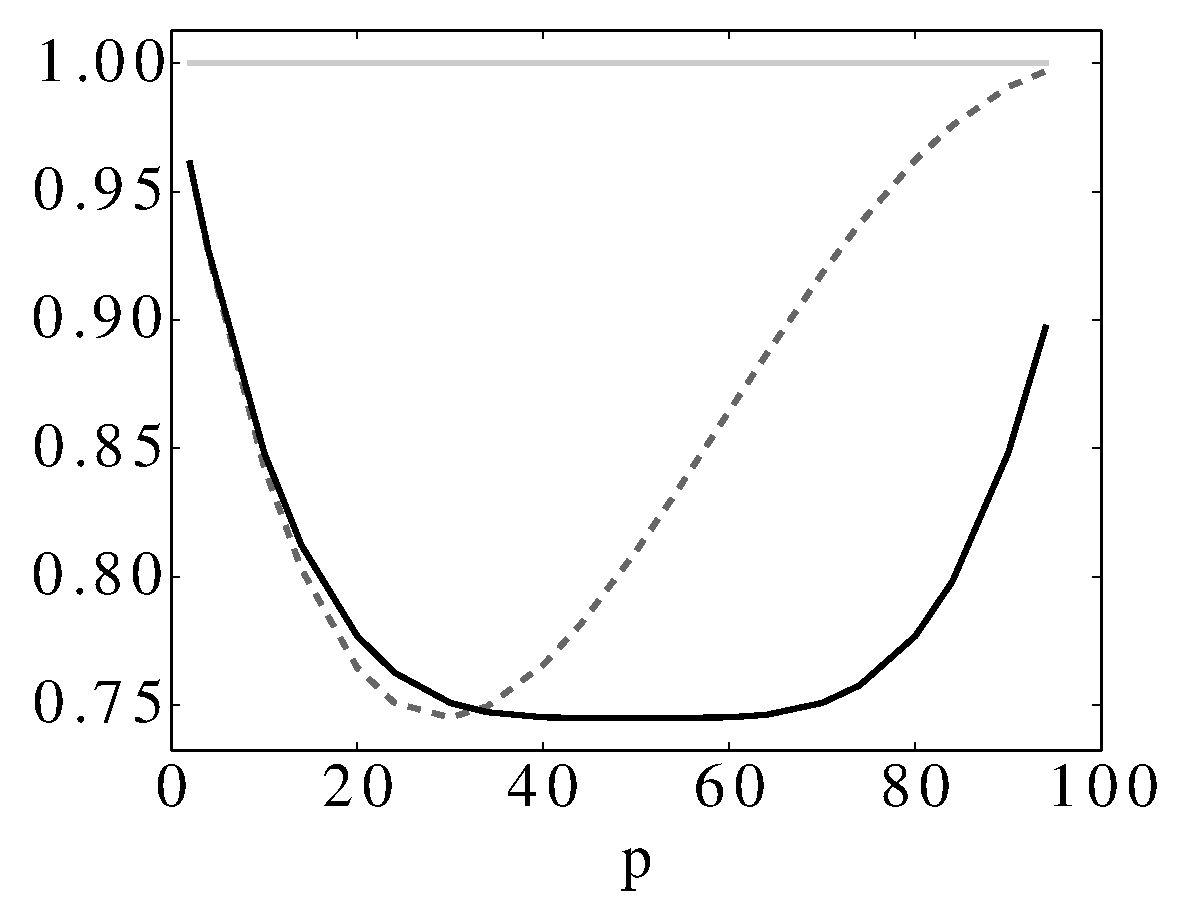
\includegraphics[width=\linewidth]{img/ExpectedNodes/1Clique/Clique_Partitiondensity.eps}
		\caption{\label{fig:1CAhn}\emph{Partition Density}}		
	\end{subfigure}\hspace*{1cm}
	\begin{subfigure}{0.4\linewidth}
		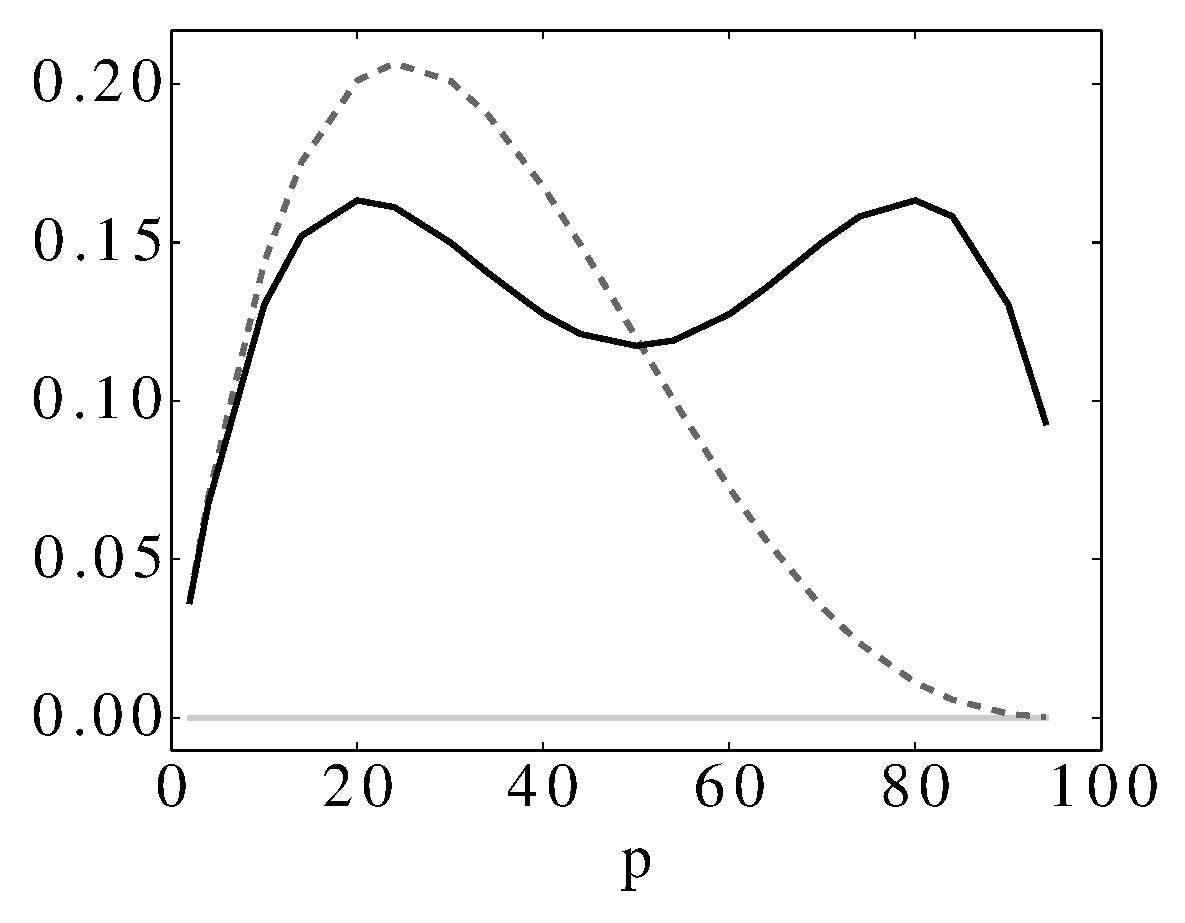
\includegraphics[width=\linewidth]{img/ExpectedNodes/1Clique/Clique_Evans1.eps}
		\caption{\label{fig:1CE2}\emph{Evans1, Evans2}}		
	\end{subfigure}

	\begin{subfigure}{0.4\linewidth}
		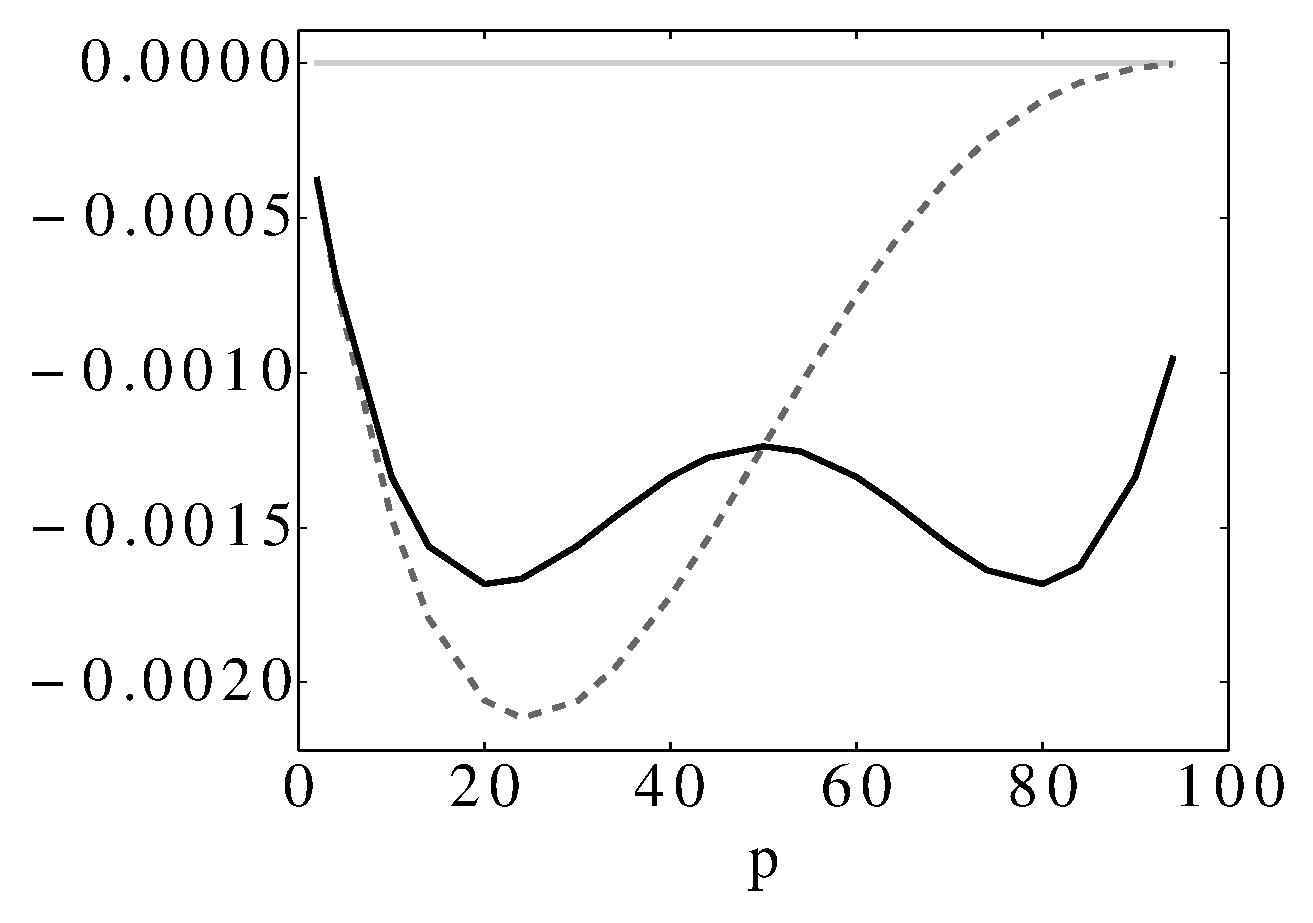
\includegraphics[width=\linewidth]{img/ExpectedNodes/1Clique/Clique_Evans3.eps}
		\caption{\label{fig:1CE3}\emph{Evans3}}		
	\end{subfigure}\hspace*{1cm}
	\begin{subfigure}{0.4\linewidth}
		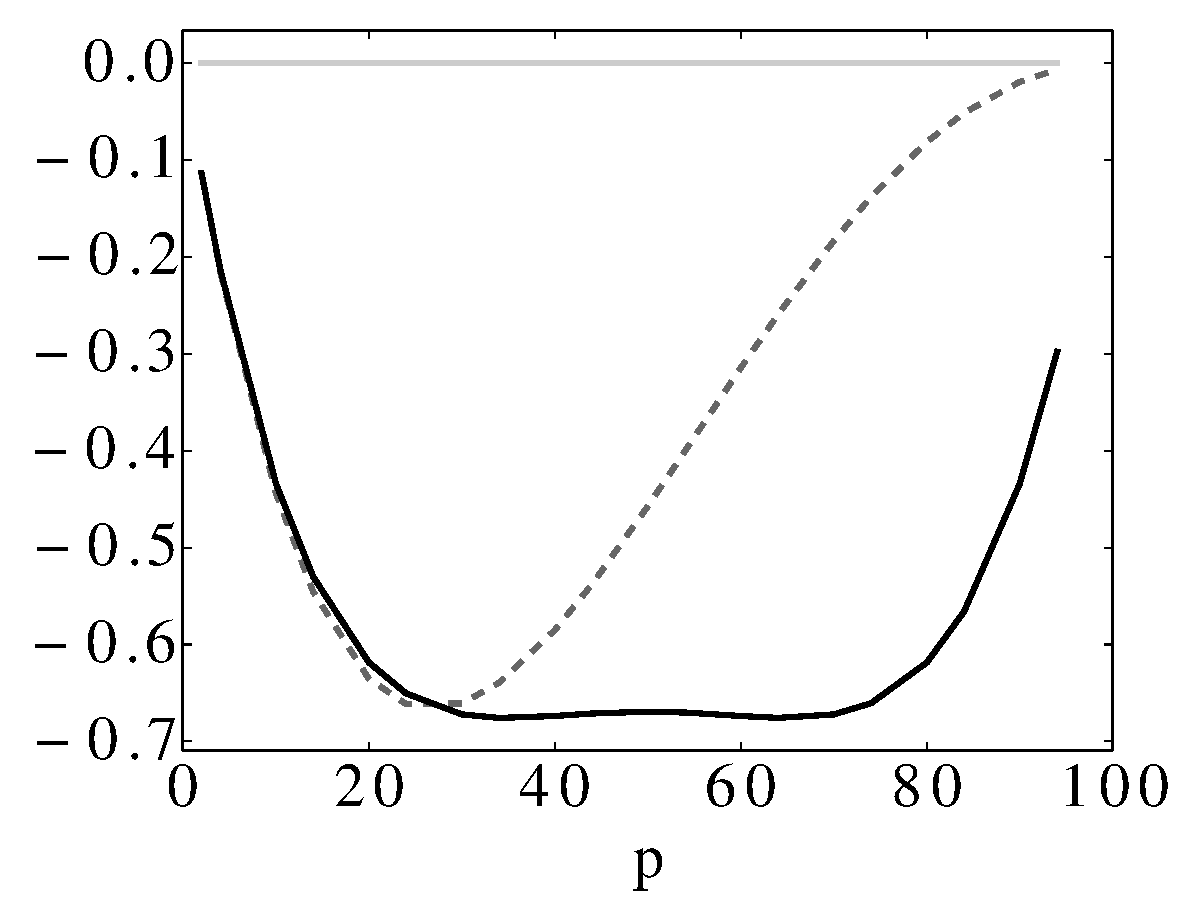
\includegraphics[width=\linewidth]{img/ExpectedNodes/1Clique/Clique_Expectednode.eps}
		\caption{\label{fig:1CMod}\emph{Expected Nodes}}		
	\end{subfigure}
		
		\caption{\`Evaluation des 5 fonctions de qualité sur un graphe complet  de $100$ n\oe uds pour trois type de partitions.
		Les partitions testées sont présentées dans la section~\ref{Completegraph}.
		Par définition, les résultats pour $Evans1$ et $Evans2$ sont identiques.
		Les lignes en gris, noir et pointillées représentent respectivement la partition triviale, les partitions en deux groupes et les partitions en trois groupes.}
		\label{fig:1Cres}
\end{figure}


\subsection{Graphe LFR}

Nous utilisons maintenant un jeu de test plus évolué.
Il n'existe pas à notre connaissance de générateur de graphe aléatoire avec une structure communautaire sur les liens.
C'est pourquoi, nous utilisons le générateur proposé par Lancichinetti~\textit{et al.}~\cite{Lancichinetti2009b}.
Ce générateur aléatoire permet de générer des graphes ayant une structure communautaire chevauchante sur les n\oe uds.
Comme nous voulons évaluer une partition de liens, il est nécessaire de transformer cette vérité de terrain.
Nous introduisons deux transformations de la couverture des n\oe uds en deux partitions de liens, $TA$ et $TB$, voir figure~\ref{fig:Trans}.


Reprenons l'exemple d'un réseau d'interactions de personnes où chaque personne appartient à différents groupes.
Afin de simplifier l'exemple, nous considérons qu'il n'existe que deux groupes: \emph{travail} et \emph{amis}.
Le but est de déterminé le type d'une interaction à partir des groupes des personnes.

Si deux personnes partagent un seul groupe, par exemple \emph{travail}, alors il est clair que l'interaction entre ces deux personnes devraient également être de type \emph{travail}.

Si deux personnes ne partagent aucune communauté, l'une est dans \emph{travail} et l'autre dans \emph{amis}, alors plusieurs choix sont possible pour le type de l'interaction.
Soit l'interaction a un type \emph{travail-amis} car on considère que toutes les interactions reliant deux personnes des groupes \emph{travail} et \emph{amis} sont de même types.
Soit l'interaction a son propre type car on considère qu'elle est unique.

Enfin, deux personnes peuvent partager plus qu'une communauté si les deux sont dans les communautés \emph{travail} et \emph{amis}.
Dans ce cas, l'interaction peut être due à l'un de ces deux groupe indépendamment.

On définit maintenant de manière plus formel cette transformation qui également illustrée dans la figure~\ref{fig:Trans}.
Soit $u,v \in V$, $C_{u,v}$ désigne l'intersection des communautés de $u$ et $v$ dans la couverture et $U_{u,v}$ désigne leur union.
Nous définissons le groupe d'un lien $(u,v) \in E$ dans $TA$ et $TB$ de la manière suivante:
\begin{description}
\item[\textbf{intra-communauté}] si $|C_{u,v}| = 1$ alors $(u,v)$ est dans la communauté $C_{u,v}$;
\item[\textbf{inter-communauté}] si $|C_{u,v}| = 0$ alors dans $TA$, $(u,v)$ appartient à sa propre communauté.
Dans $TB$, le liens appartient à la communauté $U_{u,v}$, qui contient l'ensemble des liens $(u',v')$ tel que $U_{u',v'}=U_{u,v}$;
\item[\textbf{chevauchant}] si $|C_{u,v}| > 1$ alors le lien $(u,v)$ appartient aléatoirement à une des communautés appartenant à $C_{u,v}$.
\end{description}

\begin{figure}
\centering
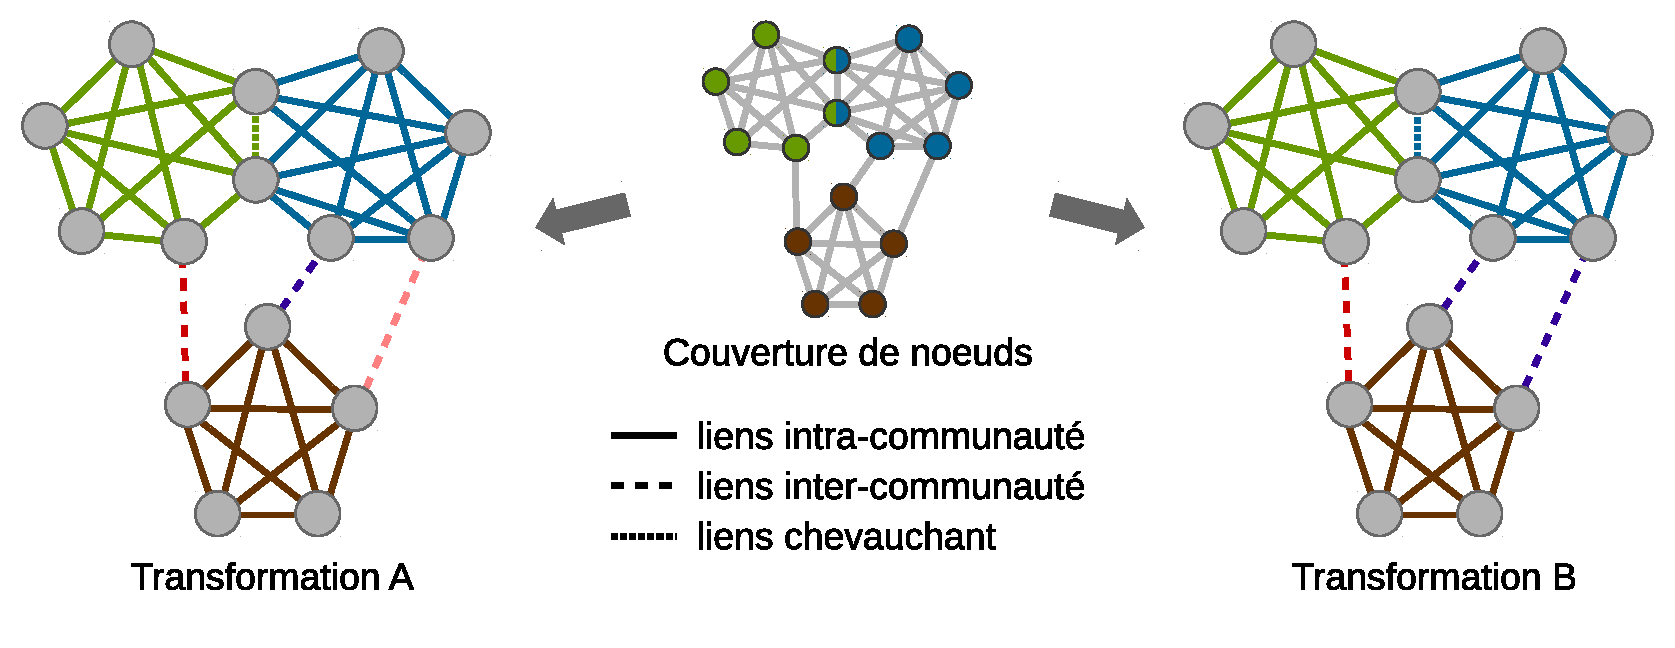
\includegraphics[width=0.9\linewidth]{img/ExpectedNodes/Example/GroundTruthTransformation}
\caption{Construction de $TA$ et $TB$ depuis une couverture de n\oe uds.
La couleur des liens indique leur groupe.}
\label{fig:Trans}
\end{figure}

Pour générer le graphe, nous avons appliqué un jeu de paramètre classiquement utilisé dans la littérature~\cite{Fortunato2010}.
Ainsi, nous avons généré des graphes de $500$ n\oe uds ayant un degré moyen de $25$, un degré max de $50$ et $10$ n\oe uds appartenant à deux communautés et des communautés ayant une taille comprise entre $20$ et $100$.
Le degré est tiré selon une loi exponentielle de paramètre $-2$ et la taille des communautés a $-1$ comme paramètre.
Enfin, 90\% des liens se sont à l'intérieur d'une communauté et les 10\% restant sont répartis de manière aléatoire.
Avec ces paramètres, il y a en moyenne $5620$ liens intra-communautés, $625$ liens inter-communauté et seulement $5$ liens chevauchant.

Pour chaque graphe généré, nous testons les partitions $TA$ et $TB$ mais aussi la partition $LC$ trouvée par \textit{link clustering}~\cite{Ahn2010a} et la partition $E2$ trouvée par la seconde méthode de Evans \textit{et al.}~\cite{Evans2009}\,\footnote{Les résultats sont similaires en utilisant $E1$ et $E3$.}.
Ces deux algorithmes optimisent respectivement \emph{Parition Density} et \emph{Evans2}.
Ces partitions sont ensuite évaluées par les fonctions de qualité \emph{Partition Density}, $Evans2$ et \emph{Expected Node}.
Une illustration d'un graphe généré et des exemples de groupes capturés par $LC$ et $E2$ sont présentés dans la figure~\ref{fig:LFR_Exemple}.

\begin{figure}
\centering
	\begin{subfigure}{0.31\textwidth}
		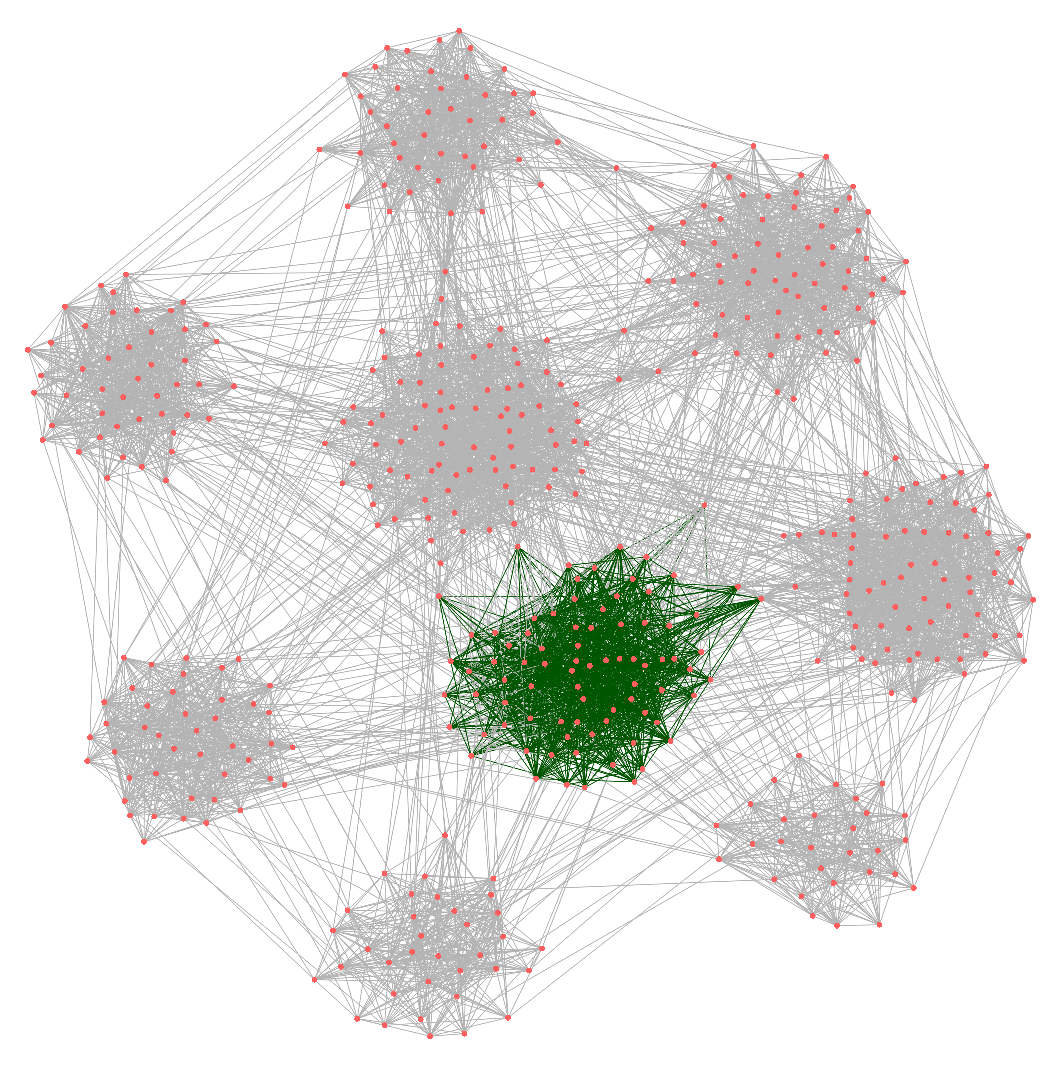
\includegraphics[width=\linewidth]{img/ExpectedNodes/LF/Graphe_Complet_select.png}
		\caption{}		
	\end{subfigure}
	\begin{subfigure}{0.31\textwidth}
		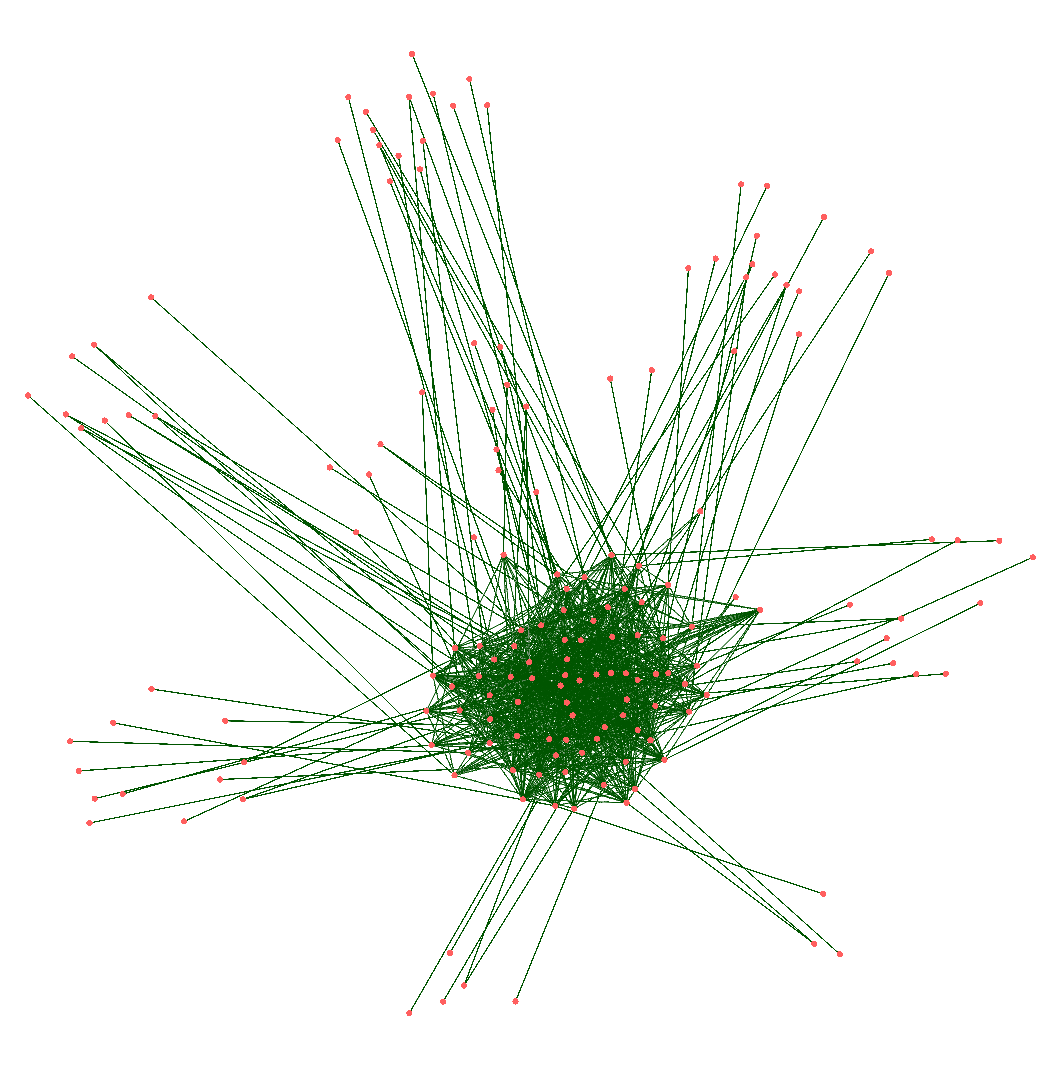
\includegraphics[width=\linewidth]{img/ExpectedNodes/LF/E2_bis.png}
		\caption{}		
	\end{subfigure}
	\begin{subfigure}{0.31\textwidth}
		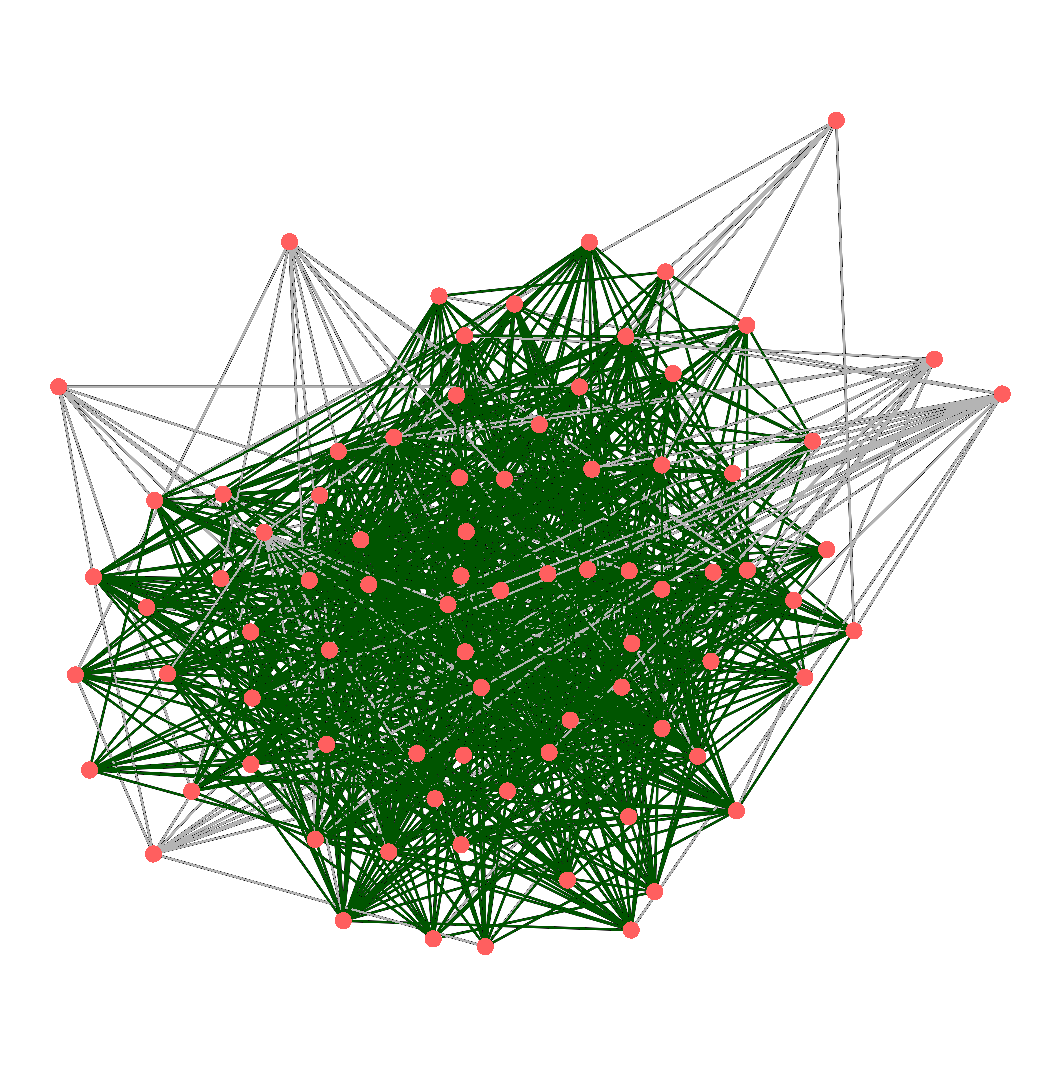
\includegraphics[width=\linewidth]{img/ExpectedNodes/LF/Ahn.png}
		\caption{}		
	\end{subfigure}

	\caption{Exemple de graphe généré par le LFR en (A) avec une communauté de la vérité de terrain mise en avant en vert.
	En (B) zoom sur une groupe détecté par $E2$ dont les liens sont en verts.
	En (C) zoom sur une groupe détecté par $LC$ dont les liens sont en verts. }
	\label{fig:LFR_Exemple}
\end{figure}


Dans $LC$, $TA$, $TB$ et $E2$, il y a $720$, $650$, $70$ et $11$ groupes en moyenne.
Afin d'observer la ressemblance de ces partitions, nous avons utilisé la NMI~\cite{Danon2005}.
Il apparait que les partitions $TA$ et $TB$ sont les plus proches.
Ensuite, nous remarquons que la partition $E2$ diffère de $TA$ et de $TB$ uniquement sur les liens inter-communautés.
En effet si ils ne sont pas pris en compte lors de la comparaison, alors $E2$, $TA$ et $TB$ sont équivalentes.
Il semble en effet que les liens inter-communautés soient arbitrairement distribués entre les plus grosses communautés adjacentes, ce qui est visible dans la figure~\ref{fig:LFR_ExempleE2}.
Enfin, la partition $LC$, bien que proche de $TA$ et $TB$, est un peu plus différente.
Ces $720$ groupes semblent plus petit mais aussi plus denses que ceux de $TA$ ou $TB$.
En particulier, les liens intra-communautés peuvent être séparés en plusieurs groupes, comme dans la figure~\ref{fig:LFR_ExempleLC}.
Les quatre partitions sont donc différentes et mettent en avant différentes caractéristiques.

Nous procédons maintenant à l'évaluation de ces partitions par les différentes fonctions de qualités.
Comme le processus de génération de graphe est aléatoire, les évaluations présentées dans la figure~\ref{fig:LF} représentent $30$ générations.
On remarque tout d'abord que ni $TA$ ni $TB$ n'a la meilleure évaluation selon $Evans2$ (figure ~\ref{fig:LFE2}) ou \emph{Partition Density} (figure ~\ref{fig:LFAhn}) même si $TA$ et $TB$ représentent nos vérités de terrain.
Dans le cas de $Evans2$, c'est la partition $E2$ qui obtient la meilleur évaluation.
Cela prouve l'efficacité de l'algorithme $E2$ pour optimiser $Evans2$ mais remet en cause la pertinence du critère $E2$ pour mettre en avant la vérité de terrain.
Notre fonction \emph{Expected Nodes} se comporte différemment des 2 autres.
Tout d'abord, c'est la vérité de terrain $TA$ qui obtient la meilleure évaluation puis il s'agit de $TB$ ou $LC$ selon les générations.
Notre mesure semble donc bien mettre en avant la vérité de terrain générée.
De plus, \emph{Expected Nodes} évalue différemment les partitions $TA$ et $TB$ contrairement à \emph{Partition Density} et \emph{Evans2}.
C'est un point important car, dans la partition $TB$, les liens inter-communautés peuvent donner lieu à des groupes non-connexes dans $TB$, voir figure~\ref{fig:Trans}.
Ce phénomène est très pénalisé par \emph{Expected Nodes}.
Enfin selon \emph{Expected Nodes}, la partition $E2$ est une mauvaise partition et cela est également dù aux liens inter-communautés.
En effet en les fusionnant à une communauté adjacente, cela augmente fortement le nombre de n\oe uds interne ce qui fait baisser $Q_{in}$.

Avec ce test, nous mettons en évidence les limites des fonctions de qualités existantes.
Les fonctions de qualité $Evans_x$ ne peuvent pas permettre de capturer les vérités de terrain généré par LFR.
En effet, l'algorithme de Louvain est capable de trouver une partition ayant une évaluation plus élevé que la vérité de terrain.
La \emph{Partition Density}, quant à elle, souffre surtout de son incapacité à différencier clairement des partitions différentes.
Cela se matérialise par des évaluations très similaires pour les vérités de terrain et la partition $LC$.
Il en résulte que la \emph{Partition Density} est sensible aux faibles perturbations.
Lors de ces tests, \emph{Expected Nodes} ne semble pas souffrir de ces défauts.
Pour ces raisons, nous pensons que \emph{Expected Nodes} est une mesure qui permet de bien évaluer les partitions de liens.

\begin{figure}
\centering
	\begin{subfigure}{0.31\textwidth}
		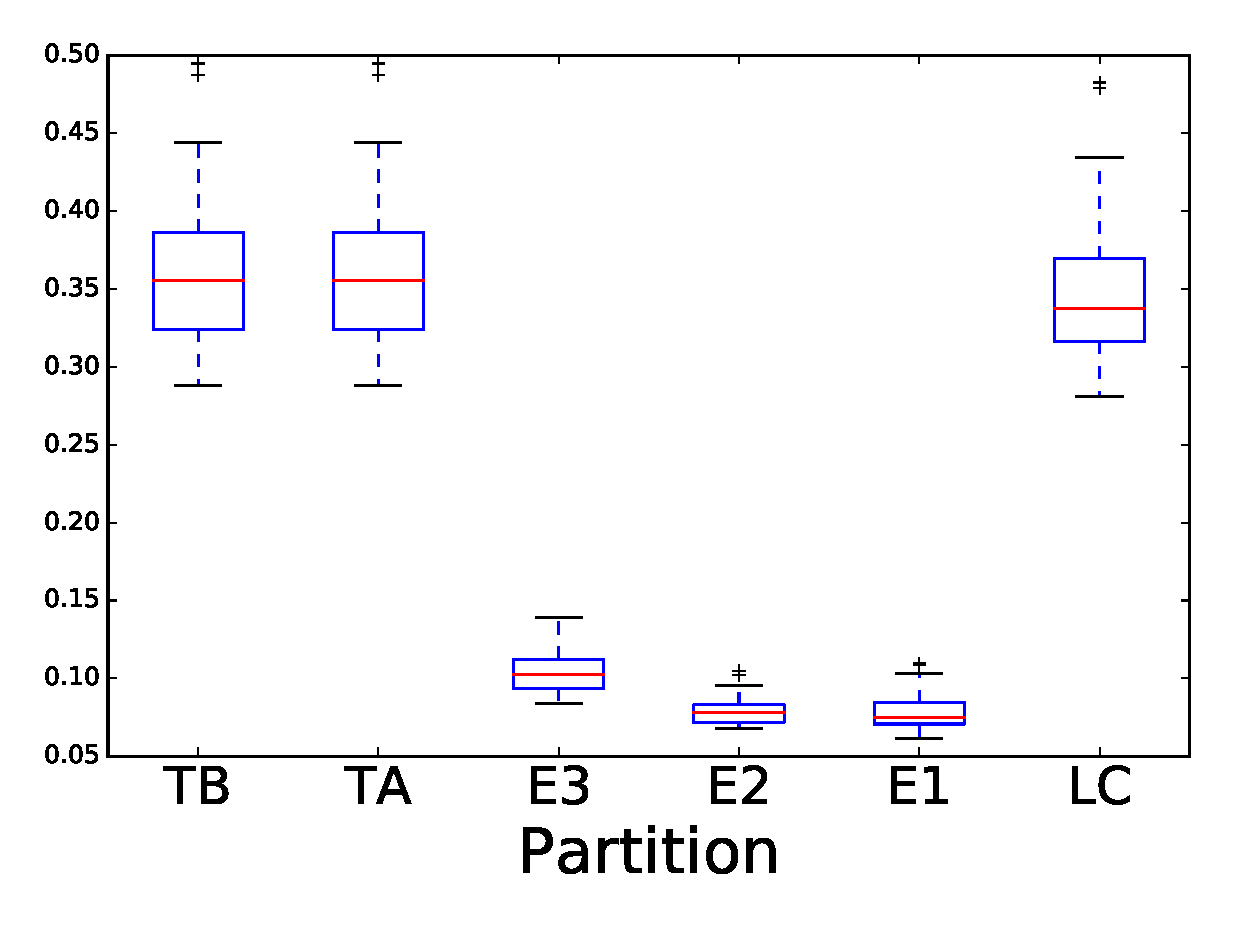
\includegraphics[width=\linewidth]{img/ExpectedNodes/LF/LFR1_Partitiondensity_ALL.eps}
		\caption{\label{fig:LFAhn}Partition density}		
	\end{subfigure}
	\begin{subfigure}{0.31\textwidth}
		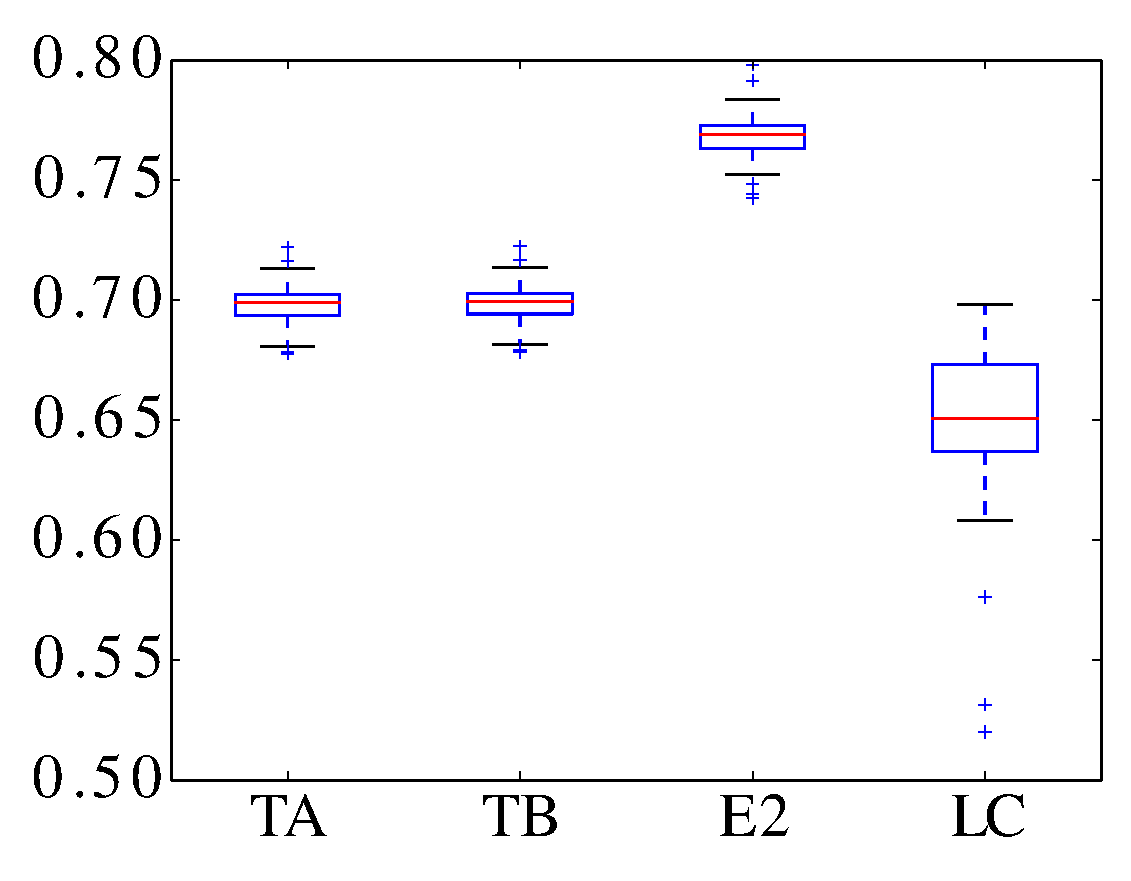
\includegraphics[width=\linewidth]{img/ExpectedNodes/LF/LFR1_Evans2_ALL.eps}
		\caption{\label{fig:LFE2}Evans2}		
	\end{subfigure}
	\begin{subfigure}{0.31\textwidth}
		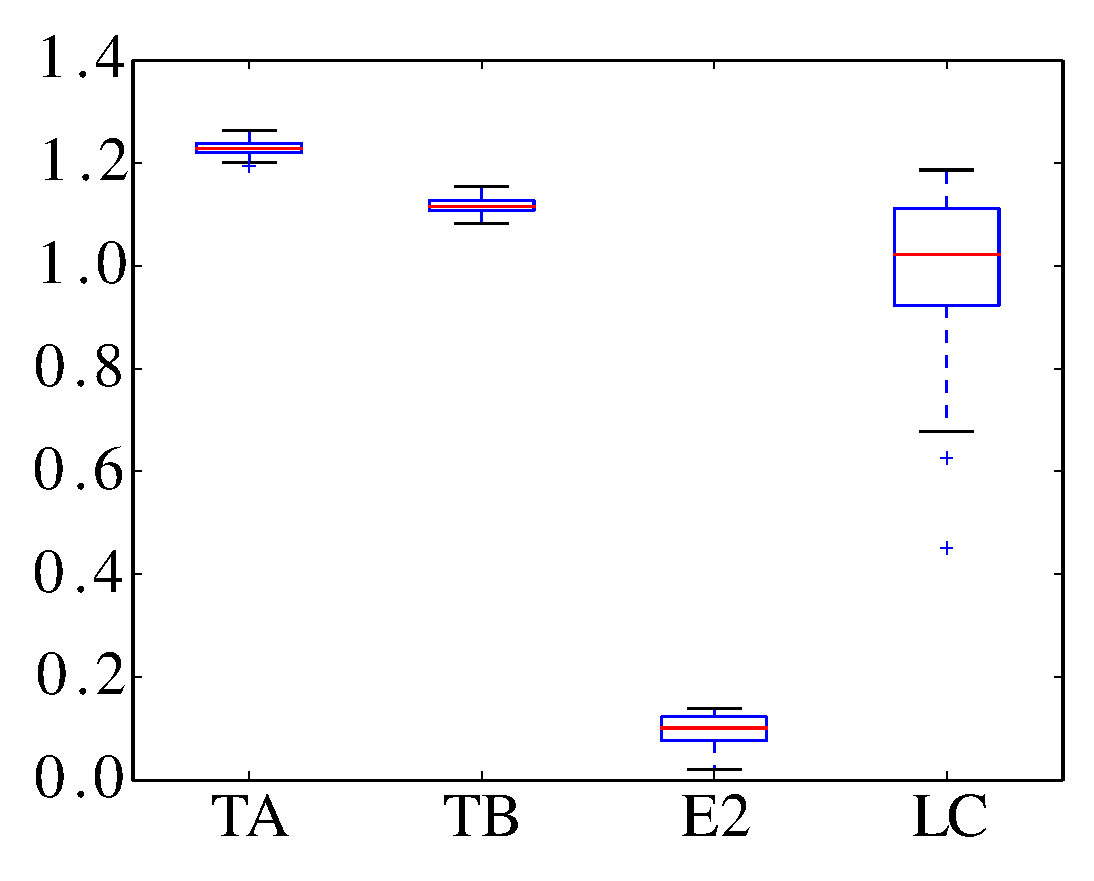
\includegraphics[width=\linewidth]{img/ExpectedNodes/LF/LFR1_ExpectedNodes_ALL.eps}
		\caption{\label{fig:LFMod}Expected Nodes}		
	\end{subfigure}
	\caption{Boite à moustache des évaluations des trois fonctions de qualité pour les différentes partitions de liens. 
	La boite représente le premier et troisième quartile ainsi que la médiane.
	Les moustaches s'étendent sur $1.5$ fois l'écart interquartile. 
	Les croix sont les points au delà des moustaches.
	}
	\label{fig:LF}
\end{figure}


\section{Calcul et optimisation}
Jusqu'à maintenant, nous avons évalué \emph{Expected Nodes} sans nous attacher ni à son calcul ni à son optimisation.
Nous discutons maintenant de la complexité de calcul d'\emph{Expected Nodes} pour une partition donnée.
Le calcul de la qualité interne \ref{eq:qin} nécessite d'évaluer la probabilité qu'un n\oe ud soit tiré.
Ce calcul de probabilité nécessite d'évaluer pour un n\oe ud $u$: $1 - \dfrac{ \binom{2|E|-d(u)}{2|L|} }{ \binom{2|E|}{2|L|} }$, ce qui peut être assez couteux.
Ce calcul correspond à une loi hypergéométrique.
Or sous certaines conditions, une loi hypergéométrique peut être approché par une loi binomiale ce qui simplifie le calcul à: $1 - (1- \dfrac{|L|}{|E|})^{|L|}$ ce qui est plus rapide.
Lors de nos tests, le biais induit par cette approximation reste assez faible, de l'ordre de $0.01\%$ en moyenne.
Ce changement de calcul est équivalent à considérer un tirage avec remise au lieu de tirage sans remise.
De plus cette probabilité ne dépend que du degré du n\oe ud et du nombre de liens dans le groupe.
Donc, tout les n\oe uds ayant le même degré donnent lieu à la même probabilité.
Si l'on considère que l'évaluation de la probabilité pour un n\oe ud peut se faire en $O(1)$ alors, pour un groupe donné, il est possible de calculer sa qualité en $O(|\{d_G(v)\}_{v \in V}|)$.
Cette formulation est très efficace lorsque beaucoup de n\oe uds ont le même degré.
Enfin comme la qualité d'un groupe ne dépend que de sa taille, on peut calculer la qualité d'une partition $\mathcal{L}$ en $O(\{|L_i|\}_{L_i \in \mathcal{L}})$.

Il est donc assez rapide de calculer $Q_{in}$.
En revanche, la situation est complètement différente pour $Q_{ext}$.
Le processus de calcul est similaire.
On peut également appliquer l'approximation de la loi hypergéométrique par une loi binomiale mais deux n\oe uds de même degré ne vont plus forcément avoir la même probabilité d'être tirés.
En effet, $Q_{ext}$ n'utilise pas le graphe initial mais le graphe $G\setminus L_i$.
Pour chaque n\oe ud, il faut évaluer son degré dans ce nouveau graphe.
Le calcul de $Q_{ext}$ pour un groupe se fait donc en $O(n)$.
Pour l'évaluation d'une partition, il n'est pas non plus possible de considérer comme équivalents des groupes de même taille.
Le coût pour évaluer une partition est donc en $O(|\mathcal{L}|n)$.
Le code pour évaluer une partition de liens d'un graphe avec \emph{Expected Nodes} mais aussi avec \emph{Partition Density}, $Evans1$, $Evans2$ et $Evans3$ est disponible en ligne: \url{https://github.com/ksadorf/ExpectedNodes}.


Malgré ce coût élevé, nous avons développé un premier algorithme d'optimisation glouton de \emph{Expected Node}.
Le principe de fonctionnement est le suivant.
Chaque lien est initialement dans son propre groupe.
Puis à chaque itération, on considère deux types de modification de la solution courante.
Soit la meilleure fusion de deux communautés soit le meilleur changement de communauté d'un seul lien.
On fusionne ou change de communauté un lien si cela améliore la qualité de la partition.
Les fusions considérées sont les fusions entre des communautés adjacentes.
Les changement de liens se font également que avec une communauté adjacente.
On continue de modifier la solution courante tant qu'elle est améliorable par un de ces mouvements.
Malheureusement cette approche souffre de deux problème majeurs.
Tout d'abord le calcul du gain est couteux et rend impossible l'étude de grands jeux de données.
Ensuite dans nos tests dans les graphes généré par LFR, il semble que cette méthode reste bloquée sur des optimum locaux bien plus faibles que la vérité de terrain.
Il faudrait donc tester d'autres heuristiques d'optimisation mais aussi travailler sur une méthode de calcul du gain plus optimisée.

Malgré ces limitations, nous avons tout de même tiré parti de cet algorithme naïf afin de tester si une partition donnée peut être améliorée.
En effet même si l'algorithme n'est pas adapté pour trouver une partition ayant une qualité élevée en partant de zéro, il peut modifier une partition donnée pour l'améliorer. 
Nous avons donc utilisé les partitions $TA$ et $TB$ comme partition de départ de l'algorithme et nous avons observé si l'algorithme est capable d'améliorer les vérités de terrain.
Les changements qu'apportent notre algorithme se porte principalement sur les liens inter-communautés.
Dans le cas de $TA$, chaque lien inter-communauté constitue une communauté.
Or, il se peut que plusieurs liens inter-communautés soient connectés aux même n\oe uds.
Dans ce genre de situation, notre algorithme fusionne ces liens dans une communauté augmentant légèrement la qualité globale.
Après optimisation, nous constatons que les partitions $TA$ et $TB$ peuvent être légèrement améliorées mais qu'elles sont très proche du maximum local lorsque l'on considère notre algorithme d'optimisation.


\section{Conclusion}

Nous considérons de nouveaux critères pour l'évaluation des partitions de liens tenant compte de la répartition des n\oe uds internes et externes d'un groupe.
\`A partir de ces critères, nous définissons une mesure de qualité, \emph{Expected Nodes}, basée sur la différence entre le nombre de n\oe uds induits par un groupe de lien et le nombre de n\oe uds attendu dans un modèle nul.
Ce processus est similaire à celui qui a donné lieu à la modularité.
En plus de s'inspirer de la modularité, \emph{Expected Nodes} ne prends pas uniquement en compte la répartition de ses n\oe uds induits mais également celle de n \oe uds et liens adjacents.
Ce changement permet d'avoir une évaluation plus fine d'une communauté.
Pour montrer la pertinence de cette nouvelle fonction de qualité, nous évaluons quatre fonctions de qualité de la littérature.
Nous montrons que, sur nos jeux de tests, \emph{Expected Nodes} semble être la plus à même de capturer la vérité de terrain et de différencier des partitions différentes.
Malgré le coût de calcul élevé d'\emph{Expected Nodes}, nous avons implémenté un premier algorithme d'optimisation agglomératif.
Cet algorithme n'est, pour l'instant, pas capable d'obtenir des partitions avec des scores élevés.
Cependant il nous a permis de vérifier que les vérités de terrain généré par LFR sont des quasi-optimum locaux selon \emph{Expected Nodes}.
Bien qu'il soit possible d'améliorer légèrement les vérités de terrains, la structure de l'optimum local est très proche de la partition initiale.


\subsection{Perspective}

Les perspectives autour d'\emph{Expected Nodes} sont nombreuses et portent sur deux points: d'une part le calcul et l'optimisation d'\emph{Expected Nodes} et d'autre part les cas d'applications possibles.

\subsubsection{Amélioration de l'optimisation d'\emph{Expected Nodes}}

\paragraph{Considérer plus de modifications}
Il semble que les mouvement envisagés pour modifier une solution courante ne soient pas suffisant pour échapper à des maximums locaux qui sont bien inférieurs à la qualité des vérités de terrain.
Il faudrait donc en envisager de nouveaux.
Inclure la possibilité de diviser une communauté en deux ne semble pas envisageable car ils existent de trop nombreuses coupes possible et le coût de calcul associé est trop couteux.
Il semble, par contre, prometteur de considérer des mouvements associés à un n\oe ud.
En effet au lieu de changer un à un les lien d'une communauté, il devrait être possible d'intégrer en un seul mouvement tous les liens adjacents qui sont reliés à un n\oe ud adjacent donné.
Pour l'illustrer ce mouvement, reprenons l'exemple d'une clique incluse dans une autre clique plus grande.
La solution finale devrait être la clique maximal.
Si l'on ne considère que l'ajout de lien un à un\,\footnote{Dans le cas où la fusion de communauté n'est pas une option viable.}, alors il n'est pas possible d'atteindre la clique maximal.
L'algorithme est bloqué car l'ajout d'un unique lien détériore la solution courante.
Si on considère l'ajout de tous les liens adjacents à un n\oe ud adjacent donné, alors, après l'ajout, le groupe considéré est toujours une clique et la qualité interne ne diminue pas mais en plus on peut espérer faire diminuer la pénalisation de la qualité externe.
De cette manière, il devrait être possible d'éviter des maximums locaux.
Plus globalement, les mouvement faisant intervenir plusieurs liens d'un seul coup semblent intéressants.



\paragraph{Diminuer le coût de calcul du gain}
Ici, il ne s'agit pas d'améliorer la performance de l'algorithme en terme de qualité obtenue par la partition trouvée par l'algorithme mais de le rendre plus rapide.
Dans sa version courante, l'algorithme est trop couteux pour traiter des graphes ayant plus de quelques dizaines de milliers de liens.
La force de l'algorithme de Louvain réside dans l'existence d'une expression analytique du gain de fusion de deux communautés qui est rapide à évaluer.
Dans notre algorithme, la lenteur est justement due au calcul du gain qui est très coûteux.
En effet, nous ne calculons pas directement le gain d'un mouvement mais la différence entre la qualité courante et la qualité résultant du mouvement.
C'est une différence importante car, dans notre cas, il faut calculer de zéro la qualité des communautés impactées.
Une manière de résoudre ce problème serait de ne pas partir de zéro mais de calculer localement les changements ayant un impact.
Prenons le cas de la fusion de communautés $A$ et $B$.
Cela est simple pour la qualité interne car elle ne dépend que du nombre de n\oe uds et liens internes.
Le nouveau nombre de liens, après fusion, est simplement la somme des liens des communauté initiales.
Le nouveau nombre de n\oe uds internes est la taille de l'union des n\oe uds internes.
La situation est plus complexe pour la qualité externe.
Le nouveau nombre de liens adjacents n'est pas simplement une somme.
De même, l'identité et le degré des nouveaux n\oe uds adjacents dans $G \setminus (A \cup B)$ ne sont pas triviales à calculer.
Il faudrait des parcours locaux sur $(A \cup B)$ et son voisinage pour arriver à mettre à jours ces données nécessaires au calcul de $Q_{ext}$. 
Si ce parcours est fait suffisamment soigneusement, il est surement possible de gagner en terme de vitesse d'exécution.


\paragraph{Changer la stratégie d'optimisation}
Une autre source potentielle de gain en vitesse de l'algorithme est la stratégie d'optimisation.
Lors d'une itération, nous appliquons la meilleur fusion de communauté ou le meilleur changement de communauté d'un lien.
Appliquer le meilleur mouvement peut améliorer la convergence de l'algorithme vers l'optimum local mais cela est coûteux car lors d'une itération tous les gains doivent être calculés.
C'est problématique car c'est justement le calcul du gain qui est très coûteux.
Une solution face à ce problème est d'utiliser une variante stochastique de l'algorithme.
Dans cette variante, ce n'est pas le meilleur changement qui est appliqué mais le premier qui mène à une amélioration de la qualité.
Pour ce faire, il est nécessaire de considérer un ordre aléatoire des mouvements possibles et d'appliquer le premier dont le gain est positif puis de recommencer.
Avec ce changement, on teste beaucoup moins de mouvements avant d'en appliquer un.
Cependant, il est possible que plus de mouvements soient nécessaires avant d'arriver à un optimum local.
Par ailleurs avec ce changement, l'algorithme n'est plus déterministe car il dépend de l'ordre d'évaluation des mouvements.
Il faudrait donc être très prudent vis-à-vis de ses aspects, lors du test de cette technique.

\subsubsection{Cas d'utilisation d'\emph{Expected Nodes}}
Nous avons parlé de moyens possible pour trouver une méthode d'optimisation efficace d'\emph{Expected Nodes}.
Il est également nécessaire de revenir sur l'utilisation d'\emph{Expected Nodes}.
Nous avons testé \emph{Expected Nodes} sur un algorithme largement utilisé dans la littérature et les résultats sont encourageants.
Il y a cependant une différence majeur dans la manière dont nous avons testé \emph{Expected Nodes} vis-à-vis des autres fonctions de qualités.
Il n'existe pas, pour l'instant, d'algorithme efficace pour trouver une partition maximisant \emph{Expected Nodes}.
C'est pourquoi nous testons des partitions trouvées empiriquement par d'autres moyen.
Cependant, il existe peut être une partition que nous n'avons pas testé qui aurait une bien meilleur qualité que les vérité de terrains.
L'amélioration de l'algorithme d'optimisation et le test d'autres partition accroitraient la pertinence des partitions testées et ainsi le bien fondé d'\emph{Expected Nodes}.
De manière analogue, il serait intéressant d'évaluer \emph{Expected Nodes} sur des jeux de données ayant une réelle vérité de terrain sur les liens, que ce soit des données réelles ou simulées.
Plus globalement, il serait intéressant de comprendre ce qu'il est possible de capturer et représenter comme structure avec une partition de liens.

Nous avons parlé jusque maintenant de l'application d'\emph{Expected Nodes} sur des graphes non pondérés et non dirigés.
La question de la pondération est délicate à prendre en compte pour \emph{Expected Nodes}.
En effet, notre méthode repose sur des tirages aléatoires de demi-liens.
La notion de tirage est intrinsèquement lié à des valeurs entières.
En effet, il n'existe pas à ma connaissance de pendant continue à la loi hypergéométrique;
on ne tire pas aléatoirement $0.6$ demi-liens parmi $14.3$ demi liens possible.
L'application d'\emph{Expected Nodes} à un graphe pondéré semble donc compromise.
Cependant, il devrait être trivialement possible de considérer des multigraphes.
Dans les multigraphes, deux n\oe uds peuvent être relié par plus qu'un lien.
Les notions de tirages aléatoires peuvent s'adapter à ce genre graphe assez facilement.
Il y a toute fois une différence majeur lorsque l'on considère les multigraphes par rapport aux graphes classiques: les contraintes sur la partition résultat.
Dans le cas des multigraphes, il serait surement intéressant d'ajouter la contrainte que chaque communauté ne doit contenir qu'une seule occurrence d'un lien donné.
Ainsi s'il existe deux liens entre $u$ et $v$, alors ces deux liens devront être dans deux communautés différentes.